% For full compilation to get the final document
\documentclass[a4paper, 10pt]{article}

% For quick compilation without figures
%\documentclass[a4paper, 10pt, draft]{article}
\usepackage{float}
\usepackage{listings}
\usepackage{todonotes}
\usepackage{braket}
\usepackage{mathtools}
\usepackage[mathscr]{euscript}
\usepackage{amsmath, amsfonts, amssymb, amsbsy, amsthm}

\theoremstyle{plain}
\newtheorem{theorem}{Theorem}
\newtheorem*{theorem*}{Theorem}
\newtheorem{definition}[]{Definition}
\newtheorem{lemma}[]{Lemma}
\renewcommand\thelemma{\unskip}
\renewcommand\thedefinition{\unskip}
\renewcommand{\qedsymbol}{$\blacksquare$}

\usepackage{hyperref}
% \hypersetup{
%             colorlinks = true,
%             linkcolor  = blue,
%             filecolor  = magenta,
%             urlcolor   = blue
%            }
\urlstyle{same}

% Just to do labels in gnuplot, Yeah!
\usepackage{graphicx}
\usepackage{gnuplottex}
\usepackage{gnuplot-lua-tikz}


% ------------------------------------------------------------------------------
% Personal definitions
% ------------------------------------------------------------------------------
% Redefining the \abs and \norm so that they automatically change their size
\DeclarePairedDelimiter\abs{\lvert}{\rvert}%
\DeclarePairedDelimiter\norm{\lVert}{\rVert}%

% Swap the definition of \abs* and \norm*, so that \abs and \norm resizes the
% size of the brackets, and the starred version does not.
\makeatletter
    \let\oldabs\abs
    \def\abs{\@ifstar{\oldabs}{\oldabs*}}
%
    \let\oldnorm\norm
    \def\norm{\@ifstar{\oldnorm}{\oldnorm*}}
\makeatother
% ------------------------------------------------------------------------------


%opening
\title{Thermalisation of Ultracold Bose Gases on Optical Lattices}
\author{Nikolas M. Mitchell}

\begin{document}

\maketitle

\begin{abstract}
\todo{rewrite this when rest done, David/Danny ignore the abstract for now please}
    Systems of ultra-cold gases in light-induced periodic potentials (optical
    lattices) are of great experimental and theoretical interest, and have been
    since the first experimental realisation of Bose-Einstein condensation in
    1995. This is largely due to the parallels between the behaviour of BECs in
    an optical lattice and condensed matter systems, where electrons can be
    modelled as moving on a lattice generated by the periodic array of atom
    cores \cite{Bloch2012}. This project investigates the time evolution of a
    system of bosons prepared in a far-from-equilibrium state on a
    one-dimensional or two-dimensional optical lattice. The main focus is on
    determining how the tunnelling energies and the strength of the
    interparticle interactions influence whether or not the system exhibits
    relaxation to a thermal state. For systems in which revival to the initial
    state occurs regularly (those which don't thermalise), a method for
    calculating the revival period is developed. For the systems which exhibit
    thermalisation, we attempt to characterise the long term states using [ETH,
    entropy of entanglement, whatever I actually end up doing].
\end{abstract}

\section{Introduction}
\todo{see square brackets}
[Want to include some of the stuff from section \ref{DraftFromDanny} at the 
start here]
The question of how, and under what conditions, closed quantum systems approach 
thermal equilibrium is an old question that forms the basis of a large and
active field of research. Thermalisation is well understood in the context
of classical mechanics, where it is understood \todo{I'd rather not repeat 
``understood'' twice in same sentence.} to emerge from the chaotic 
dynamics of sufficiently unconstrained systems. However, the time evolution of
quantum systems is strictly linear, and \todo{hence?} they do not exhibit chaotic 
dynamics. Nonetheless, there are a number of closed quantum systems in which 
thermalisation is observed, in the sense that the systems relax to states in 
which the values of macroscopic quantities are stationary, universal with 
respect to widely differing initial conditions, and predictable using 
statistical mechanics \cite{Rigol2008}. 

This project investigates the time evolution of a variety of different systems
composed of noninteracting and interacting bosons on one-dimensional and 
two-dimensional optical lattices that are prepared in far-from-equilibrium 
states. These systems are investigated analytically where possible, and with
numerical methods for larger and more complicated systems where an analytic 
approach is not tractable. We focus primarily on gaining a strong 
understanding of smaller systems of few lattice sites and bosons, as these
can be solved exactly. From here, we look at some larger systems with a more
approximate method that revolves around using an adaptive Runge-Kutta method
to evolve the system wavefunction according to the Gross-Pitaevskii equation.
We then look for similarities in the results of the simulations run according 
to each method to see what similarities in behaviour are retained as we move 
from small, exactly solved systems to large, numerically approximated systems.

\newpage
\section{Experiments with optical lattices}

This project considers the thermalisation behaviour of systems of bosons on 
optical lattices. One of the main factors that make these systems interesting
to work with are the deep similarities between the Hamiltonians of systems that 
can be generated using bosons on an optical lattices and those of electrons
moving on a lattice potential produced by a periodic array of atom cores. We can 
simulate these condensed matter systems with ultracold atoms by using optical 
lattices to generate the periodic potential. An optical lattice is produced by 
overlapping multiple laser beams and making use of the interference pattern. 
The alternating bright and dark areas of the interference pattern act as a 
periodic potential on the atoms through the optical dipole 
force \cite{Bloch2012}. By superimposing different
combinations of laser beams at particular frequencies and amplitudes, any
lattice geometry that can be constructed via Fourier synthesis can, in
principle, be produced \cite{Bloch2012}. This fine degree of control over the
lattice parameters, in conjunction with the ability to tune the strength of
interparticle interactions by manipulating Feshbach resonances \cite{Chin2010},
makes ultracold bosons on optical lattices an excellent arena in which to
explore various model Hamiltonians for condensed matter systems and quantum
optics.
\begin{figure}[bh!]
    \begin{center}
        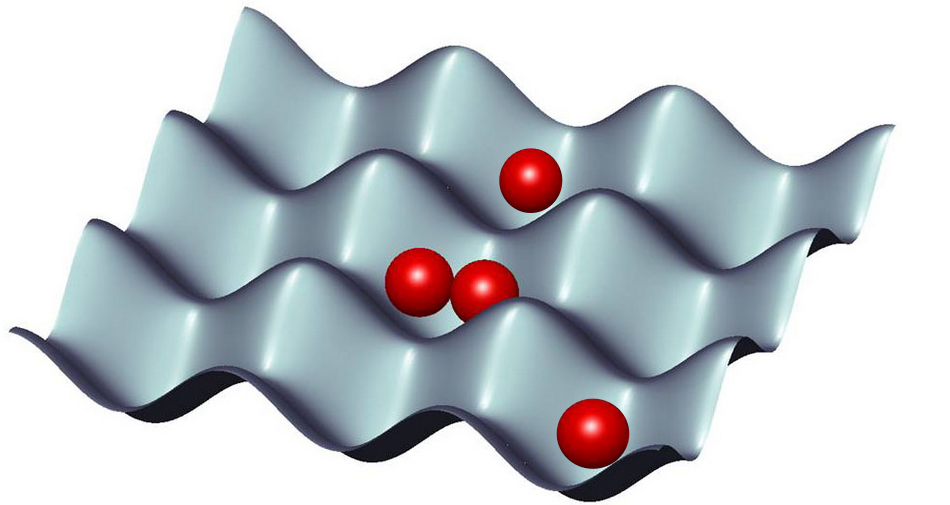
\includegraphics[width=8cm]{bosons_on_lattice}
    \end{center}
    \caption{Bosons on a two-dimensional optical lattice. Figure is taken from\newline
             \texttt{www.uibk.ac.at/th-physik/qo/research/opticallattices.html.en}
            }
\end{figure}
There are further advantages which can make conducting experiments with
ultracold bosons on optical lattices more attractive than working with solids
directly. One is that there are always impurities present in the solids we find
in nature. These impurities can have significant impacts on the properties of
the solid which cannot necessarily be accounted for by a perturbative approach
which assumes these effects to be small. \todo{reference this at some point from
the book I meant to get from David} For large-enough detunings from an atomic
transition frequency, optical lattices can be considered to be purely 
conservative and defect-free potentials \cite{Bloch2012}, so when dealing with 
bosons on optical lattices this problem of impurities does not arise.

Another benefit of working with bosons on optical lattices is that we can easily
control the state of each of the particles on the lattice. Furthermore, the
potential can be altered or switched off entirely during the experiment, which
is a feature that is not available in any solid state experiment
\cite{Morsch2006}.


\section{First quantised representation}

This dissertation will deal exclusively with bosons on optical lattices, and not
investigate cases involving fermions. There are a number of different
contributions to the Hamiltonian for bosons on optical lattices, and these
contributions can be seen to have analogues in condensed matter systems. The
individual bosons will have kinetic energy, and the potential created by the
lattice also contributes to how the system evolves in time, so it must feature
in the Hamiltonian. The bosons may be interacting, and there may also be an
external potential imposed that can vary in strength from site to site.

With regards to the interparticle interactions, we consider repulsive scattering
interactions. We will consider systems that are dilute, in the sense that the
average spacing between bosons is much greater than the effective range of the
interparticle interactions. This makes it reasonable to consider only
two-particle scattering events and neglect the rare higher order collisions,
provided we keep the strength of the interparticle interactions small. Even when
reduced to its two-body form, $U(x,x')$, the form of the interatomic scattering
potential has short range terms that can be difficult to deal with. We can
replace this object with a mathematically more convenient effective potential,
corresponding to contact interaction, with the same scattering cross-section at
low-energy. Because the ultracold bosons have such low energy, $s$-wave
scattering dominates, and the interparticle interaction potential can be
expressed simply in terms of the $s$-wave scattering length, $a_{s}$, as
\begin{equation}
    U_{\text{eff}}
    =
    \frac{2 \pi\hbar^{2} a_{s}}{m}
    \sum_{i,j}{\delta(x_{i} - x_{j})}.
\end{equation}
For simplicity, we will introduce the notation $U_{0} = \frac{4 \pi \hbar^{2}
a_{s}}{m}$. Having made these simplifications, we can construct a first
quantised Hamiltonian for a one-dimensional system of interacting bosons on an
optical lattice, in the presence of an external potential $V_{\text{ext}}$
\begin{equation}
    \label{eq:HamiltonianCoordinateRepresentation}
    \hat{h}
    =
    \sum_{i}{-\frac{\hbar^{2}}{2m}  \partial_{x_{i}}^{2}} +
    \sum_{i}{V_{\text{lattice}}(R_{i})} +
    V_{\text{ext}}(x) +
    \frac{U_{0}}{2} \sum_{i,j}{\delta(x_{i} - x_{j})}.
\end{equation}
Similar Hamiltonians are frequently used to describe systems of electrons on
atomic lattices. To promote conciseness, we introduce the abbreviations
\begin{equation*}
    \hat{h}_{1}
    =
    \sum_{i}{-\frac{\hbar^{2}}{2m} \partial_{x_{i}}^{2}} +
    \sum_{i}{V_{\text{lattice}}(R_{i})},
    \quad
    \hat{h}_{\text{ext}}
    =
    V_{\text{ext}}(x),
    \quad
    \hat{h}_{\text{int}}
    =
    \frac{U_{0}}{2} \sum_{i,j}\delta{(x_{i}-x_{j})}
\end{equation*}
so that $\hat{h}=\hat{h}_1+\hat{h}_{\text{ext}}+\hat{h}_{\text{int}}$.


\section{Effect of indistinguishability}

The Hamiltonian in the previous section would act on a bosonic many-particle
wave function. A single particle wave function $\psi(\mathbf{r})$ is defined
within a Hilbert space $\mathcal{H}$, which is the space of complex, square
integrable functions. It must satisfy $\int{d^3\mathbf{r}
\abs{\psi(\mathbf{r})}^{2}} < \infty$. A wave function that represents the state
of $N$ indistinguishable particles, $\psi(\mathbf{r}_{1}, \mathbf{r}_{2}, \dots,
\mathbf{r}_{N})$ is defined within $\mathcal{H}^N$, where $\mathcal{H}^N$ is
constructed as the tensor product $N$ single-particle Hilbert spaces:
\begin{equation}
    \mathcal{H}^{N} =
    \mathcal{H} \otimes \mathcal{H} \otimes \dots \otimes \mathcal{H}.
\end{equation}
The wave functions in this space are also subject to normalisation constraints,
i.e.,
\begin{equation*}
    \int d^{3} \mathbf{r}_{1} d^{3}\mathbf{r}_{2} \dots d^{3}\mathbf{r}_{N}
        \abs{\psi(\mathbf{r}_{1},\mathbf{r}_{2},\dots,\mathbf{r}_{N})}^{2}
    < \infty.
\end{equation*}
Whilst all functions satisfying the above constraints can be legitimately
defined mathematically, only a small subset are found to occur in nature --
those which are either entirely symmetric or anti-symmetric under particle
exchange. The set of indistinguishable particles which are entirely symmetric
under particle exchange are called bosons. This project will not investigate
scenarios involving the particles that display exchange anti-symmetry
(fermions), so we will be working within the space $S_{N}\mathcal{H}^{N}$. Here
$S_{N}$ projects onto the subspace of square-integrable functions that are
unchanged by permuting the order of the variables. As an illuminating example
one may construct the two-particle space, $S_{2}\mathcal{H}^{2}$ for bosons as
\begin{equation*}
    S_{2} \mathcal{H}^{2}
    =
    \left \lbrace
        \psi \mid \psi = \psi_{1} \otimes \psi_{2} + \psi_{2} \otimes \psi_{1},
        \quad \text{where }\, \psi_{1}, \psi_{2} \in \mathcal{H}
    \right \rbrace
\end{equation*}
It is apparent that $S_{2} \mathcal{H}^{2} \ne \mathcal{H} \otimes \mathcal{H}$
since in this case we would be able to distinguish particles or states.
We can formally extend this notion of exchange symmetry for larger systems and
express the requirement of exchange symmetry for bosonic systems as
\cite{Negele1988}
\begin{equation*}
    \psi({\mathbf{r}_{\mathcal{P}_1}, \mathbf{r}_{\mathcal{P}_2}, \dots,
          \mathbf{r}_{\mathcal{P}_N}})
    =
    \psi(\mathbf{r}_{1}, \mathbf{r}_{2}, \dots, \mathbf{r}_{N}),
\end{equation*}
where $\lbrace \mathcal{P}_{1}, \mathcal{P}_{2}, \dots, \mathcal{P}_{N} \rbrace$
represents any permutation, $\mathcal{P}$, of the set $\lbrace 1, 2, \dots, N
\rbrace$.

Let us first consider the case of two indistinguishable bosons. We have not yet
determined the energy eigenstates of our Hamiltonian, but if we suppose we have
the set of normalised single-particle wave functions $\lbrace \ket{\lambda}
\rbrace$, and we have one boson in state $\ket{\lambda_1}$ and another in state
$\ket{\lambda_2}$, then we can write the two-particle wave function as
\begin{equation}
    \psi(\mathbf{r}_{1},\mathbf{r}_{2})
    =
    \frac{1}{\sqrt{2}}
    \big (
        \braket{\mathbf{r}_{1} | \lambda_1} \braket{\mathbf{r}_{2} | \lambda_2} +
        \braket{\mathbf{r}_{1} | \lambda_2} \braket{\mathbf{r}_{2} | \lambda_1}
    \big ),
\end{equation}
or in Dirac bra-ket notation, the two-body states would be represented as
\begin{equation}
    \ket{\lambda_1, \lambda_2}
    =
    \frac{1}{\sqrt{2}}
    \big (
        \ket{\lambda_1} \otimes \ket{\lambda_2} +
        \ket{\lambda_2} \otimes \ket{\lambda_1}
    \big ).
\end{equation}

The number of permutations that one must account for grows extremely quickly as
particle number increases. A properly symmetrised and normalised $N$-body state
can be represented \cite{Altland2010} as
\begin{equation}
    \ket{\lambda_{1}, \lambda_{2}, \dots, \lambda_{N}}
    =
    \frac{1}{\sqrt{N! \prod_{\lambda = 0}^{\infty}{n_{\lambda}}}}
    \sum_{\mathcal{P}}
        \ket{\lambda_{\mathcal{P}_{1}}} \otimes
        \ket{\lambda_{\mathcal{P}_{2}}} \otimes
        \dots                         \otimes
        \ket{\lambda_{\mathcal{P}_{N}}},
\end{equation}
where $n_{\lambda}$ is the number of particles in state $\lambda$, and the
summation runs over all $N!$ permutations $\mathcal{P}$ of the set of quantum
numbers $\lbrace \lambda_{1}, \dots, \lambda_{N} \rbrace$.

This formalism has a number of shortcomings. The most important of these for
this project is that it is extremely cumbersome for practical computation
because of the large number of entities that need to be represented. To avoid
this, we shall adopt the second quantised formalism, which is much better suited
to dealing concisely with large numbers of indistinguishable particles.
\newpage


\section{Second Quantisation}

\subsection{The Occupation Number Representation}

The formalism that we have hitherto discussed explicitly represents a
significant amount of redundant information, in the sense that it deals
separately with the scenarios ``particle 1 in state $\lambda_1$ and particle 2
in state $\lambda_{2}$'' and ``particle 2 in state $\lambda_1$ and particle 1 in
state $\lambda_{2}$''. Taking into account the indistinguishability of the
particles, it is clear that these two scenarios are identical. A more efficient
approach consists of describing the number of particles in a particular state
$\lambda_i$, i.e., using the occupation number representation. When doing this,
a general state can be written as a linear superposition
\begin{equation}
    \ket{\Psi}
    =
    \sum_{n_{1}, n_{2}, \dots}%
        {c_{n_{1}, n_{2}, \dots}\ket{n_{1}, n_{2}, \dots}}.
\end{equation}
In the scenario which this project will be working with, the occupation numbers
refer to the number of bosons on a particular site of the lattice. Having
established this, we can define creation and annihilation operators that create
and annihilate particles from number eigenstates, that is
\begin{equation}
    \hat{a}_{j}^{\dagger} \ket{n_{1}, n_{2}, \dots, n_{j}, \dots}
    =
    \sqrt{n_{j} + 1} \ket{n_{1}, n_{2}, \dots, n_{j}+1, \dots}
\end{equation}
and
\begin{equation}
    \hat{a}_{j} \ket{n_{1}, n_{2}, \dots, n_{j}, \dots}
    =
    \sqrt{n_{j}} \ket{n_{1}, n_{2}, \dots, n_{j}-1, \dots}.
\end{equation}
These operators have very important commutation relations
\begin{equation}
    [ \hat{a}_{j}^{\dagger}, \hat{a}_{k}^{\dagger}] = 0, \quad
    [ \hat{a}_{j}, \hat{a}_{k}]=0, \quad
    [\hat{a}_{j},\hat{a}_{k}^{\dagger}]=\delta_{jk}.
\end{equation}
We can also define the number operator $hat{n}_{j} = \hat{a}_{j}^{\dagger}
\hat{a}_{j}$ that has the property that
\begin{equation}
    \hat{n}_{j} \ket{n_{1}, n_{2}, \dots, n_{j}, \dots}
    =
    n_{j} \ket{n_{1}, n_{2}, \dots, n_{j}, \dots}.
\end{equation}

The occupation number eigenstates form the basis of the $N$-particle Hilbert
space that we are working in (the Fock space $\mathcal{F}^N$), and it is useful
to observe that any occupation number eigenstate can be created from the empty
(or ``vacuum'') state $\ket{0}$ by repeated action of
creation operators \cite{Altland2010}
\begin{equation}
 \ket{n_1,n_2,\dots}=\prod_i\frac{1}{\sqrt{n_i!}}(\hat{a}_i^{\dagger})^{n_i}\ket{0}.
\end{equation}

It may seem that the state space $S_N\mathcal{H}^N$ that we have constructed is
not robust enough to accommodate these operators. Indeed, the creation and
annihilation operators take us from the $N$-particle Hilbert space to the
$(N+1)$- and $(N-1)$-particle Hilbert spaces, respectively. In order to account
for these differences in particle number, we must really be working within the
symmetric Fock states $\mathcal{F}_{S}(\mathcal{H})$, defined by the direct sum
\cite{Blank1999}
\begin{equation}
    \mathcal{F}_{S}(\mathcal{H}) = \oplus_{N=0}^\infty S_{N} \mathcal{H}^N.
\end{equation}

However, we will be working in systems in which the particle number is
conserved. Each combination of creation and annihilation operators that appears
in the Hamiltonian will create an equal number of particles to the number
destroyed. So for practical purposes we are just working within $S_{N}
\mathcal{H}^{N}$.

Having established the space and states that we are operating with, we now need
to rewrite the Hamiltonian in number state representation, i.e., we need to
``second quantise'' it.


\subsection{Second Quantisation of the Hamiltonian}

We can second quantise the Hamiltonian initially used to describe our system
through the boson field operators, $\hat{\psi}^{\dagger}(x)$ and
$\hat{\psi}(x)$, which create and destroy particles at particular spatial
locations (we will define these more explicitly later). The two terms in
$\hat{h}_1$ are single-particle operators for the kinetic and potential energy
contributions, and can be transformed to
\begin{equation}
    \hat{H}_{1}
    =
    \int{\hat{\psi}^{\dagger}(x) \hat{h}_{1} \hat{\psi}(x) \,dx}.
\end{equation}

The one-dimensional Bloch's theorem states \cite{Bloch1929, Kittel1987} that the
eigenstates of a particle in a periodic potential have the form
\begin{equation}
    \phi_{q}(x) = e^{iqx} u_{q}(x),
\end{equation}
where $q$ is the quasi-momentum and $u_{q}(x)$ is periodic with the same period
as the lattice, $d$. We will be considering scenarios in which the strength of
the lattice potential is such that the bosons are not completely localised, but
such that the overlap between the wave functions of particles on particular
lattice sites have effectively zero overlap with non-nearest neighbours. Under
these conditions, the wave functions can be conveniently described by the
localised Wannier functions
\begin{equation}
    \psi(R;r) = \frac{1}{d} \int{dq\, e^{iRq} \phi_{q}(x)}
\end{equation}
which are superposition of Bloch functions \cite{Kittel1987, Wannier1937}. This
is a useful description because the Wannier functions are both orthonormal and,
more importantly, complete. We can use this to rewrite the field operators as
\begin{equation}
    \label{field_operators_wannier}
    \hat{\psi} = \sum_{j}{\hat{a}_{j}\psi(R_{j} - x)}.
\end{equation}
\todo{Time-dependence in $a$?}
With this in mind, we can write
\begin{equation}
    \int{
         \sum_{j}{\hat{a}_j^{\dagger}\psi^{*}(R_j-x)}
         \hat{h}_{1}
         \sum_{l}{\hat{a}_l\psi(R_{l} - x)}
         \,dx}
    =
    \sum_{j,l}{J_{j,l} \hat{a}_{j}^{\dagger} \hat{a}_{l}}.
\end{equation}
Here we have introduced a shorthand notation
\begin{equation}
 J_{j,l} = \int{\psi^{*}(R_{j} - x) \hat{h}_{1} \psi(R_{l}-x) \,dx}
\end{equation}
for the numerical values of these integrals. Notice that the integration --at
least numerically-- can indeed be carried out and characterises the strength of
the hopping between sites $j$ and $l$. It is typically described \todo{need
references!} as characterising the overlap of the single-particle spatial wave
functions (see figure below).
\begin{figure}[h!]
    \begin{center}
        \includegraphics[width=0.8\textwidth]{J_overlap_drawing}
    \end{center}
    \caption{\label{fig:J_overlap_drawing}
             The strength of hopping $J$ is considered as the overlap of
             localised Wannier functions centred at neighbouring lattice sites.}
\end{figure}
This is not entirely accurate, as the Wannier states are orthonormal and so the
integral over their inner product is zero. More precisely, $J_{j,l}$ takes the
inner product between a Wannier state $\psi(R_{j} - x)$ and the state produced
by the action of $\hat{h}_1$ on the Wannier state $\psi(R_{l} - x)$, which does
not have to be zero. However, the depiction in figure \ref{fig:J_overlap_drawing}
can still be useful for developing an intuition for what $J$ is, since $J$
depends on the combination of the lattice depth (and width) and the kinetic
energy and so would the overlap of the spatial wave functions if they were not
orthonormal. It is also clear from the figure that computing overlap integrals
using wave functions on non-neighbouring sites does not add much accuracy to our
model, so we neglect these. For the hopping interactions that are permitted, we
assume that each has identical strength. This assumption allows us to write
\begin{equation}
    \hat{H}_{1}
    =
    \int{\hat{\psi}^{\dagger}(x)
         \bigg(
            \!\sum_{i}{-\frac{\hbar^{2}}{2m} \partial_{x_{i}}^{2}} +
            \sum_{j}{V_{\text{lattice}}(R_{j})}
         \bigg)
         \hat{\psi}(x) \,dx}
    =
    J \sum_{i}{(\hat{a}^\dagger_{i}\hat{a}_{i+1}+h.c.)},
\end{equation}
where $h.c.$ denotes the hermitian conjugate. We can go through a similar
process for the contributions of the external potential and on-site interactions
between bosons. The external potential gives an on-site energy that can vary at
different locations in the lattice
\begin{equation}
    \hat{H}_{\text{ext}}
    =
    \int{\hat{\psi}^{\dagger}(x) V_{\text{ext}}(x) \hat{\psi}(x) \,dx}
    =
    \sum_{i}{\epsilon_{i} \hat{a}_{i}^{\dagger} \hat{a}_{i}}.
\end{equation}

The term for on-site interaction between bosons is a two-particle operator, thus
second quantisation requires integration between two sets of boson field
operators
\begin{equation}
    \hat{H}_{\text{int}} =
    \int{\hat{\psi}^{\dagger}(x) \hat{\psi}^{\dagger}(x)
          \frac{U_{0}}{2} \sum_{i,j}{\delta(x_{i}-x_{j})}
          \hat{\psi}(x) \hat{\psi}(x) dx
        }
    =
    \frac{U_{0}}{2}
    \sum_{i}
        {\hat{a}_{i}^{\dagger} \hat{a}_{i}^{\dagger} \hat{a}_{i} \hat{a}_{i}}
\end{equation}

Putting these terms together, we arrive at the Bose-Hubbard model described in
the next section.


\section{The Bose-Hubbard model}

The Hamiltonian for a weakly interacting BEC in a one-dimensional optical
lattice and subject to harmonic trapping potential is given by the sum of
$\hat{H}_{1}$, $\hat{H}_{\text{ext}}$ and $\hat{H}_{\text{int}}$:
\begin{equation}
    \hat{H}_{\text{1D}}
    =
    J \sum_{i}{(\hat{a}^\dagger_{i}\hat{a}_{i+1} + h.c.)} +
    \frac{U_{0}}{2}
    \sum_{i}%
        {\hat{a}_{i}^{\dagger} \hat{a}_{i}^{\dagger} \hat{a}_{i} \hat{a}_{i}} +
    \sum_{i}%
        {\epsilon_{i} \hat{a}_{j}^{\dagger} \hat{a}_{j}},
\end{equation}
and is known as the Bose-Hubbard Hamiltonian. The $\epsilon_{i}$'s refer to
on-site energies at each lattice site due to the harmonic trap, and the middle
term gives an interaction energy when there is more than one particle on a
particular site. This project will look at scenarios where there is no external
harmonic potential which produces different on-site energies for different sites
(the uniform lattice potential remains, so $J$ is still defined as before). In
the absence of this external potential, the Hamiltonian in one dimension reduces
to
\begin{equation}
\begin{align*}
\hat{H}_{1D}
=
&J\sum_{i}(\hat{a}^\dagger_{i}\hat{a}_{i+1}+h.c.\ )
+
\frac{U_0}{2}\sum_{i}\hat{a}^\dagger_{i}\hat{a}^\dagger_{i}
\hat{a}_{i}\hat{a}_{i}.
\end{align*}
\end{equation}

This project aims to explore the dynamics of both this one-dimensional system
and the two-dimensional version where we couple multiple chains of lattice
sites together. The system Hamiltonian in two dimensions is

\begin{equation}
\hat{H}_{2D}=\left(J\sum_{i,j}\hat{a}^\dagger_{i,j+1}\hat{a}_{i,j}
+
J'\sum_{i,j}\hat{a}^\dagger_{i,j}\hat{a}_{i+1,j}\right)+h.c.
+
\frac{U_0}{2}\sum_{i}\hat{a}^\dagger_{i}\hat{a}^\dagger_{i}
\hat{a}_{i}\hat{a}_{i},
\end{equation}
where the $i$ index denotes which chain is being referred to and the $j$ index
denotes how far along the chain a site is. $J'$ is another hopping parameter,
in this case characterising the hopping between sites on different chains.
\begin{figure}[H]
    \begin{center}
        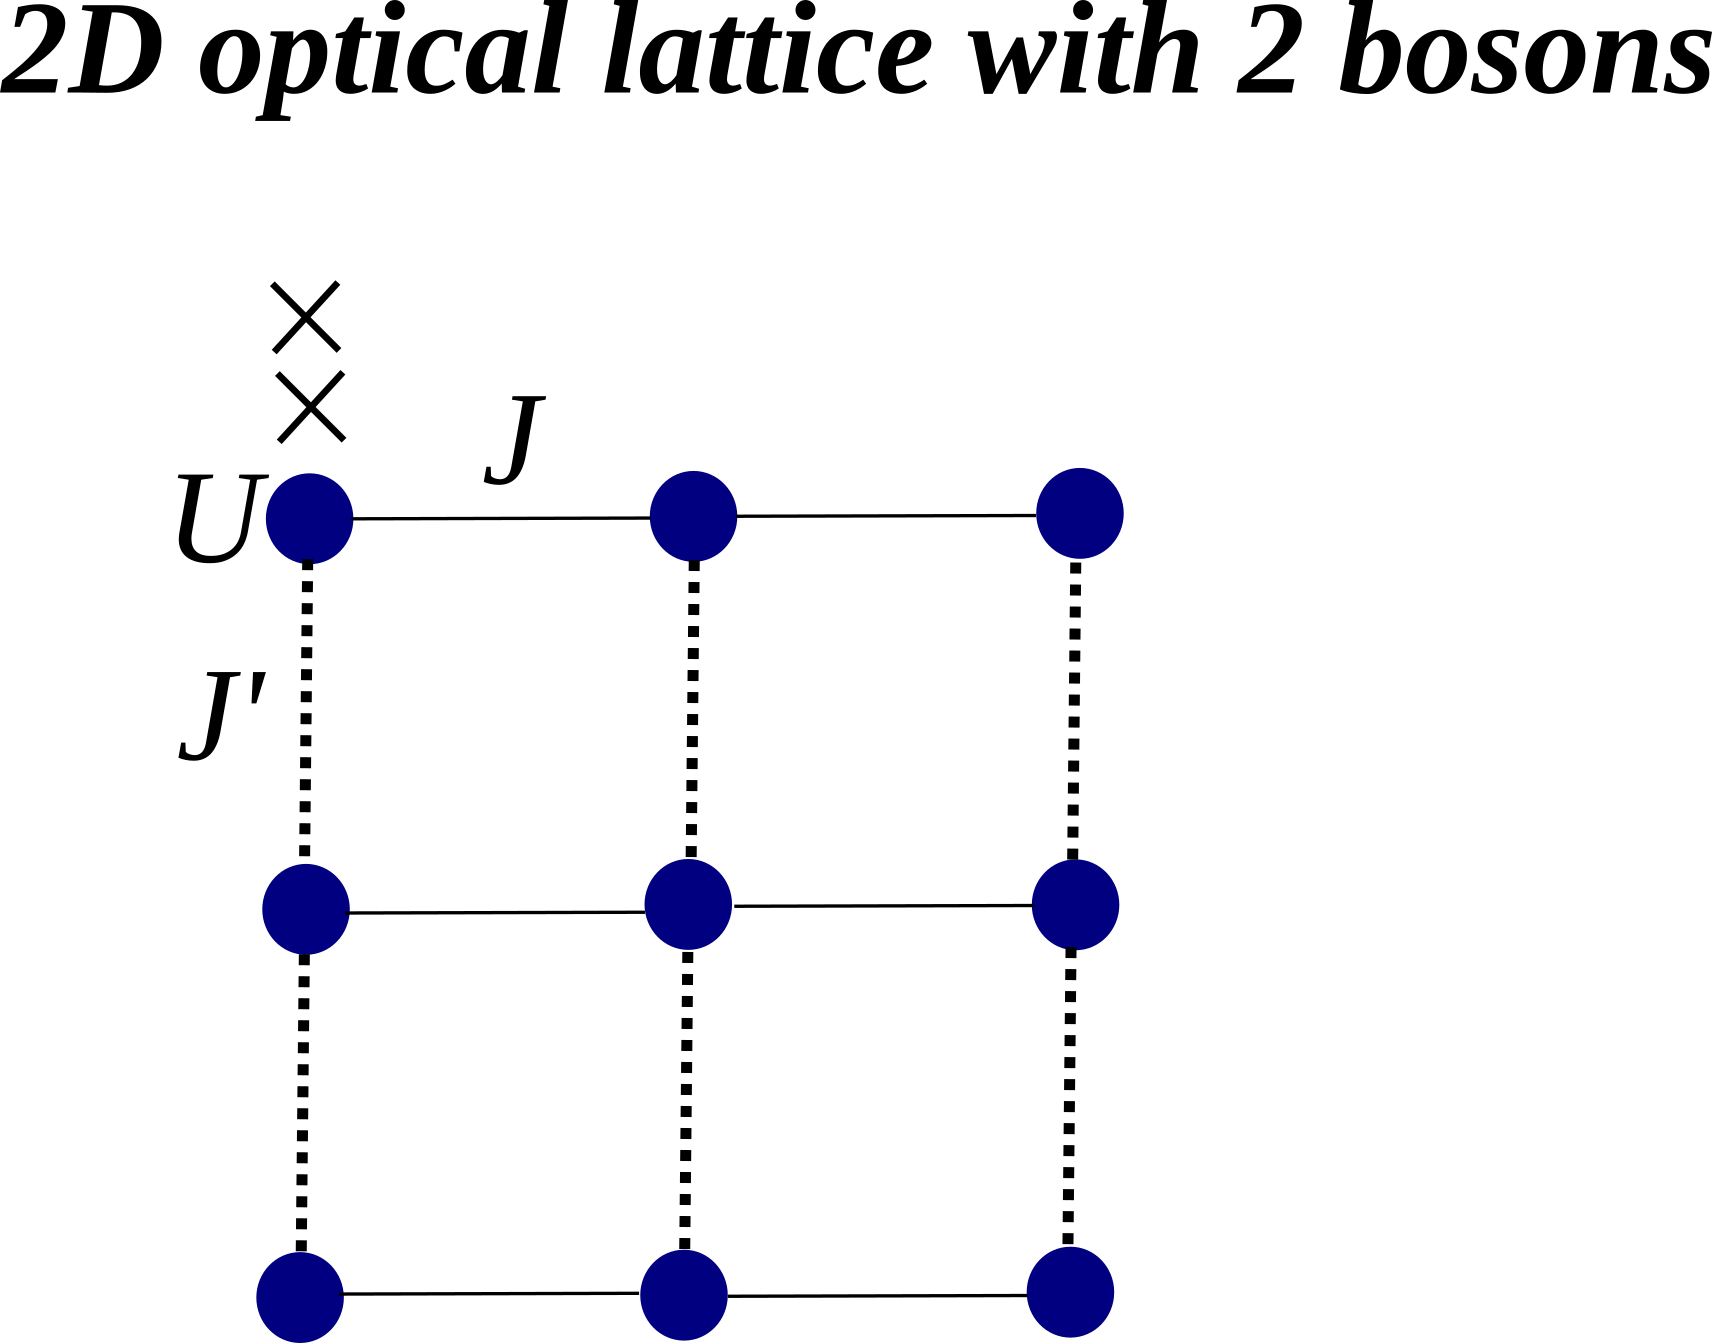
\includegraphics[width=8cm]{lattice_pic}
    \end{center}
    \caption{The blue circles here represent lattice sites and the crosses
             denote individual bosons. Hopping between any two neighbouring
             sites on the same chain is characterised by $J$, whereas hopping
             between chains is characterised by $J'$. A three by three lattice
             is shown here, but the system can be extended to arbitrary size.
            }
\end{figure}
We are interested in the time evolution of these systems as it relates to their
thermal behaviour.


\section{Thermalisation}

\subsection{Overview}

Thermalisation refers to a relaxation of a system to states where the values
of macroscopic quantities are stationary, universal with respect to widely
differing initial conditions, and predictable using statistical mechanics
\cite{Rigol2008}. We observe thermalisation in a wide variety of classical
systems, and there are strong theoretical reasons for anticipating this
thermalisation. However, many of these reasons don't apply when considering
quantum systems. The question of which, if any, quantum systems exhibit
thermalisation and how the thermal states can be characterised is of
considerable theoretical and experimental interest.

\subsection{Classical systems}

To see why thermalisation is common and even expected in many classical
systems, we need to understand the property of ergodicity and the impact of
chaotic dynamics on it. If you start an isolated system in a particular
configuration corresponding to a particular point in phase space, it can move
through that phase space along the constant-energy manifold. A system is
ergodic if the long-term time average of any single phase space trajectory
is equivalent to an ensemble average. \todo{get Kinoshita's definition
of ergodicity} \todo{Do I need to elaborate on this further?}Classical systems
exhibit chaotic dynamics, which are strongly nonlinear and allow the system to
quickly and essentially uniformly explore the constant-energy manifold
irrespective of the initial conditions. This promotes ergodicity, which is
implicit in the fundamental assumption of statistical mechanics - all
accessible microstates are equiprobable. \todo{Need to explicitly link
ergodicity and thermalisation, otherwise this is just free-floating and its
relevance is not obvious. What is this link?} This is what leads us to expect
our classical systems to thermalise.

\subsection{Draft: from Danny\label{DraftFromDanny}}

It is our everyday experience that a hot tea or coffee cools and reaches the
temperature of its surrounding, or in general when a system or its environment
undergo a change, the system of interest usually respond but after a while it
reaches a new state where no further macroscopic change takes place and an
observer may conclude that the system reached its {\emph{thermodynamic
equilibrium}}. However, this phenomenon raises the question: how does the system
approach its new equilibrium state?

While Ludwig Boltzmann developed the theory of entropy based on notions of
statistics and probability theory (L. Boltzmann: ``Weitere Studien über das
Wärmegleichgewicht unter Gasmolekülen''. [Further studies about the heat
equilibrium among gas molecules] Sitzungsberichte der Akademie der
Wissenschaften Wien (II) 66 (1872) pp. 275–370.). During the derivation of the
aesthetically pleasing relatinoship $S=k_{B}\ln{\!(W)}$ for an ideal gas
consisting of $N$ particles, Boltzmann a priori considered that each realisation
of particles is equally probable. However, the evolution of the system would
lead to a distribution of macroscopic quantities for which there are more
possible microscopic realisations.

Although Boltzmann established the connection between the micro- and macroscopic
world, even his contemporaries, e.g., Lord Kelvin (W. Thomson: ``The kinetic
theory of energy dissipation'', Proceedings of the Royal Society of Edinburgh 8
(1874) pp. 325–334.) and Johann Josef Loschmidt (Loschmidt, J., (1876/1877),
``Über die Zustand des Wärmegleichgewichtes eines Systems von Körpern mit
Rücksicht auf die Schwerkraft'', Wiener Berichte, 73: 128, 366 (1876); 75: 287;
76: 209 (1877).), raised two philosopically hard questions: reversibility and
recurrence.

The former relies on the time-reversal symmetry of classical mechanics, thus one
may expect processes with decreasing entropy occurring as often as ones which
increase the entropy of a system. We note here that the same objection cannot be
raised if one replaces classical mechanics as the description of the microscopic
world with quantum mechanics. The basic equation of non-relativistic quantum
mechanics is the Sch{\"o}dinger equation, which is {\emph{not}} invariant under
time-reveral symmetry.

The second objection was raised by Planck's student, Ernst Zermelo. His argument
was based on Henri Poincare's fresh result (H. Poincaré: ``Sur le problème des
trois corps et les équations de dynamique'' [On the three-body problem and the
dynamical equations] Acta mathematica 13 (1890) pp.1–270. See also : H. Poincaré:
``Le mécanisme et l’expérience’’ [Mechanics and experience] Revue Métaphysique
Morale 1 (1893) pp. 534–537.), namely that a mechanical system returns or almost
returns to its initial state. Zermelo argued (E. Zermelo: ``Über einen Satz der
Dynamik und die mechanische Wärmelehre'' [On a theorem of dynamics and the
mechanical theory of heat] Annalen der Physik 57 (1896) pp. 485–494.) that if
this is the case then entropy must decrease in some portion of the time
evolution.

This second argument, however, is at the heart of this dissertation as well,
since unitary time evolution forms the basis of quantum mechanics. The
incongruence between the notions of thermalisation and unitary time evolution
inspired a vibrant research field \cite{Calabrese2006, Cazalilla2006, Rigol2007,
Palma2015}. One of the emerging ideas is the {\emph{eigenstate thermalization
hypothesis}} (ETH) \cite{}. If the conditions of ETH are satisfied then it leads
to thermalisation, as it has been proven \cite{}, i.e., ETH is sufficient for
guaranteeing thermalisation. Recently G. de Palma et al. also argued
\cite{Palma2015} that ETH is also necessary for thermalisation.


\subsection{Quantum systems}
Quantum systems do not \todo{usually?} exhibit dynamic chaos \todo{see square
brackets} [Rigol's line is ``dynamical chaos itself cannot occur in an isolated
quantum system, in which the time evolution is linear and the spectrum is
discrete'' How does that argument work?], so it is not obvious how one would
justify applying the assumption of ergodicity in these systems. Because of
this, it is unclear if, or when, we should expect quantum systems to
thermalise, or what statistical ensemble we could use to characterise the
relaxed states.


\section{Integrable systems}
There are a number of classical, isolated systems that do not display
thermalisation. The main difference between these systems and those which
approach thermal equilibrium is the extent to which they are constrained
relative to the number of degrees of freedom that they possess. This observation
is formalised in the notion of integrability. A system is said to be integrable
if it has \todo{half? according to handout this seems to be the case} as
many independent integrals of motion (which are conserved) as it has degrees
of freedom. An integral of motion for a Hamiltonian is a smooth function
$I$ defined on an open subset of the phase space such that $\dot{I}=0$ on
solutions. \todo{reference handout Danny gave me, I can't see anywhere where
its from}So $I(x(t))=\text{constant}$, where $x(t)$ is the solution of the
equations of motion for a particular initial condition. If $x_1(t)$ and
$x_2(t)$ are solutions for different initial conditions, then in most cases
$I(x_1(t))\ne I(x_2(t))$. Integrability is a useful property, though it is
quite rare.

Theoretically, we can find exact solutions for the equations of motion for a
system if it is integrable, otherwise we cannot. In classical mechanics, the
idea of integrability is well-understood and neatly defined. The situation in
quantum mechanics is much more challenging. One reason for this is that
the Heisenberg uncertainty principle prevents us from applying the idea of
points in phase space with particular trajectories. With respect to the systems
that we are dealing with, it has been shown that a one-dimensional lattice
chain of non-interacting bosons is an integrable system \cite{Rigol2007}.



\todo{see square brackets} [Maybe fall back on ``All 1D systems with conserved
energy are integrable'' for U!=0, referencing page 6 of the handout Danny gave
me. I don't really know where to go for 2D at this point.]


\section{Experimental studies}

\subsection{A quantum Newton's cradle}

Kinoshita et. al. investigated \cite{Kinoshita2006} the thermalisation of an
out-of-equilibrium one-dimensional Bose gas, which is a  nearly-integrable system. They
started with several thousand arrays of one-dimensional Bose gases, each
containing from $40$ to $250$ $^{87}$Rb atoms. The atoms were trapped by
combining a blue-detuned \todo{write more about red-detuned and blue-detuned 
lasers from what I learned talking to David.} two-dimensional optical lattice, 
which provides tight transverse confinement, with a red-detuned crossed dipole 
trap providing weak axial trapping. In order
to create the non-equilibrium momentum distributions, they then pulsed on a
$3.2$ THz detuned one-dimensional lattice, which depleted the zero momentum state
and put the atoms in a superposition momentum state of $\pm2\hbar k$. The two
parts of the wave function then oscillated out of phase with each other,
colliding with each other twice every full cycle and either reflecting off
each other elastically or transmitting straight through like a ``ghostly''
Newton's cradle (see diagram below)

\begin{figure}[H]
    \begin{center}
    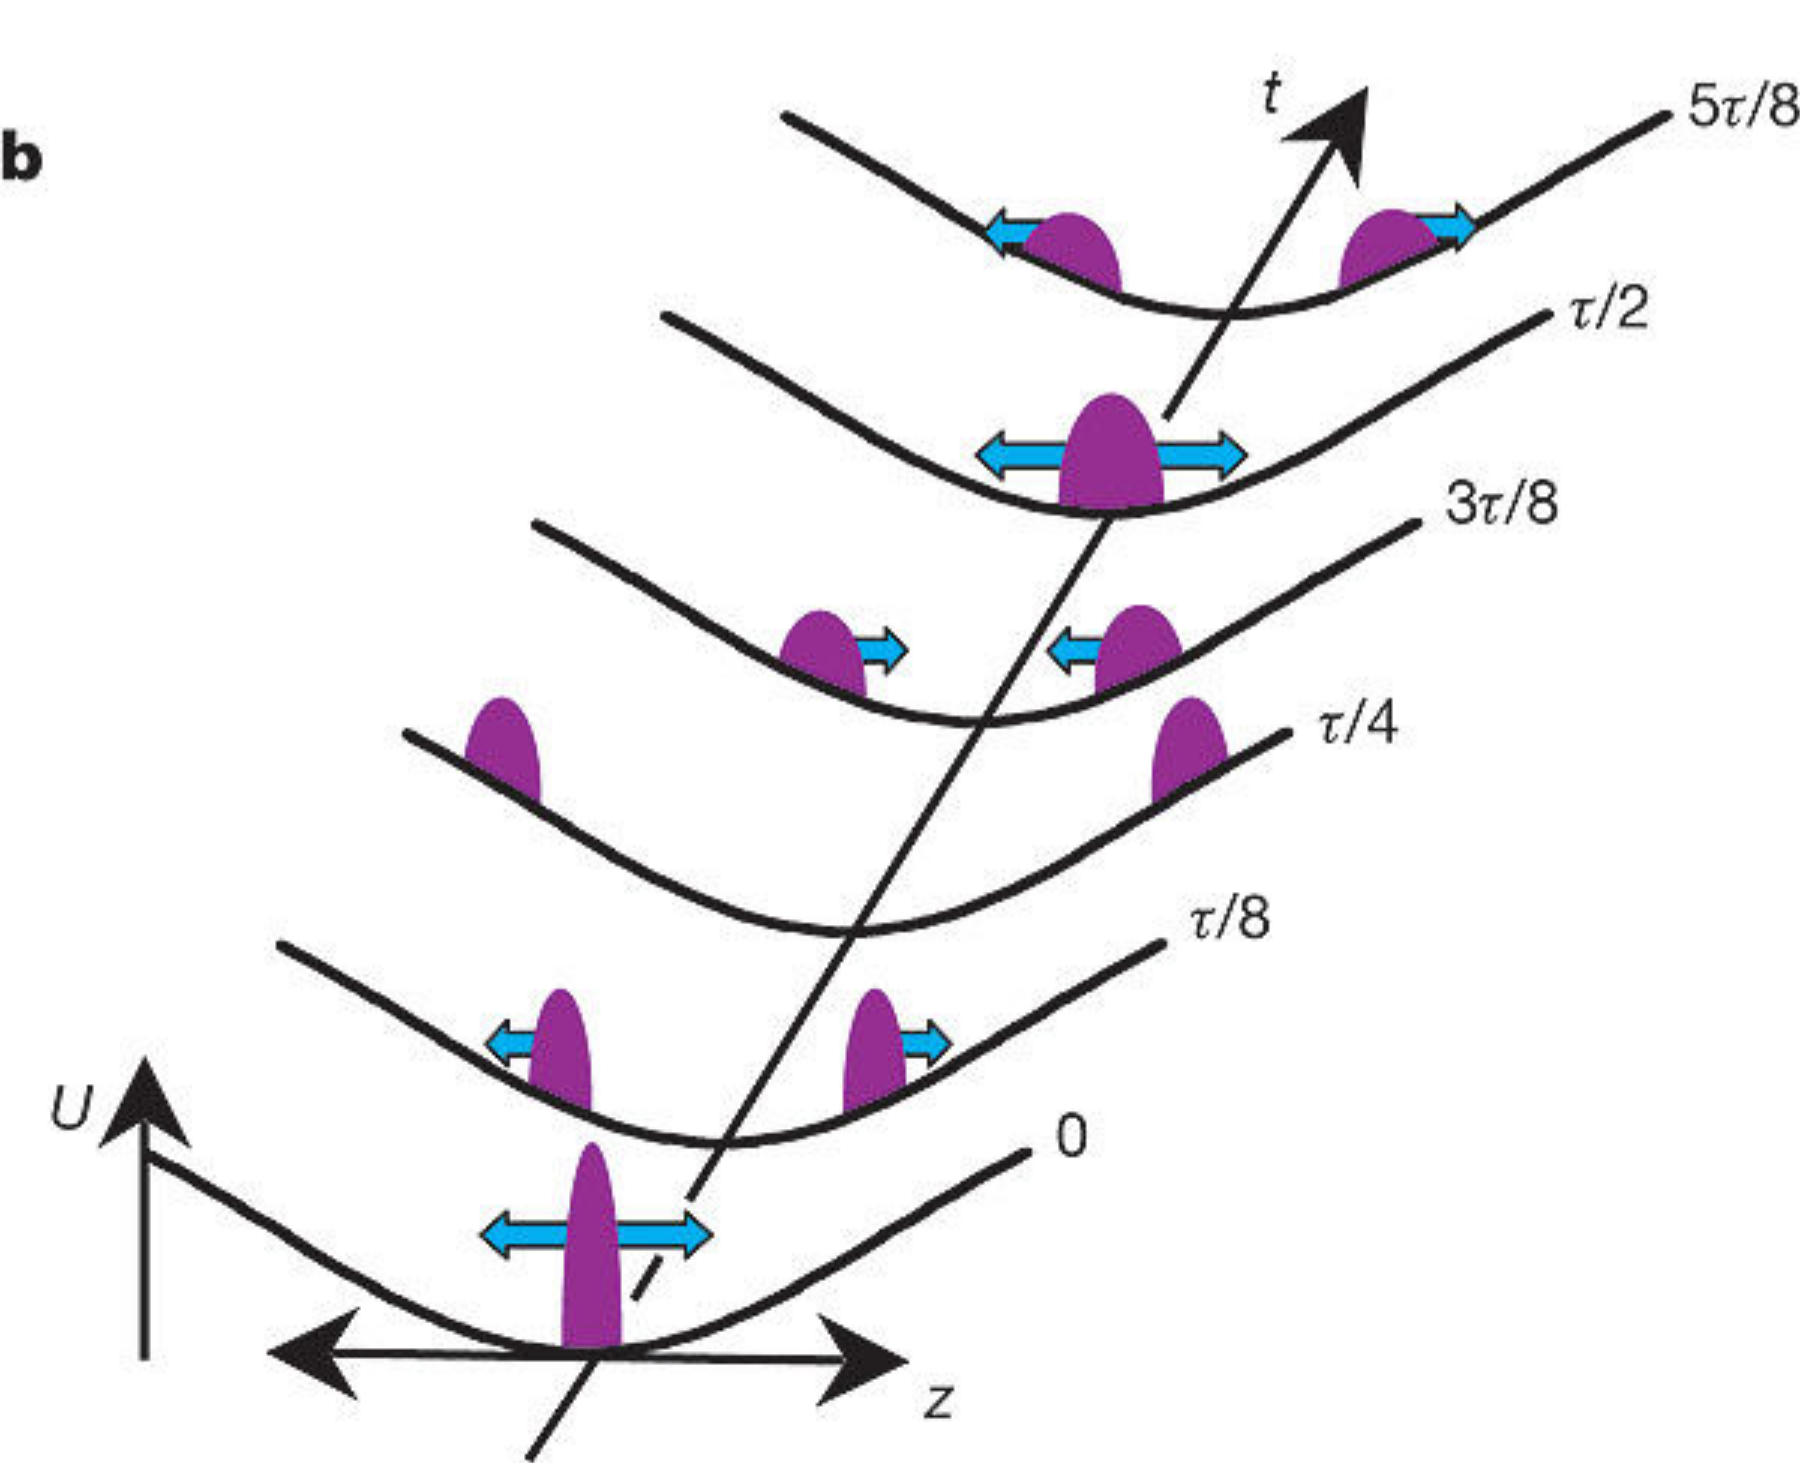
\includegraphics[width=8cm]{quantum_newtons_cradle}
    \end{center}
    \caption{Sketches at various times of two out of equilibrium clouds of atoms
             in a one-dimensional anharmonic trap. At time $t=0$ the atoms are
             put into a momentum superposition with $2\hbar k$ to the right and
             $2 \hbar k$ to the left. The two parts of the wave function
             oscillate out of phase with each other with a period $\tau$. Each
             atom collides with the opposite momentum group twice every full
             cycle, for instance, at $t=0$ and $t = \frac{\tau}{2}$. Figure is
             from reference \cite{Kinoshita2006}.}
 \end{figure}

The weak anharmonicity of the trap caused the atoms to gradually dephase.
However, the momentum distribution after dephasing was not gaussian (as one
would expect for a thermalised state), and this momentum did not noticeably
tend toward this equilibrium distribution, even after thousands of collisions.

\begin{figure}[H]
    \begin{center}
    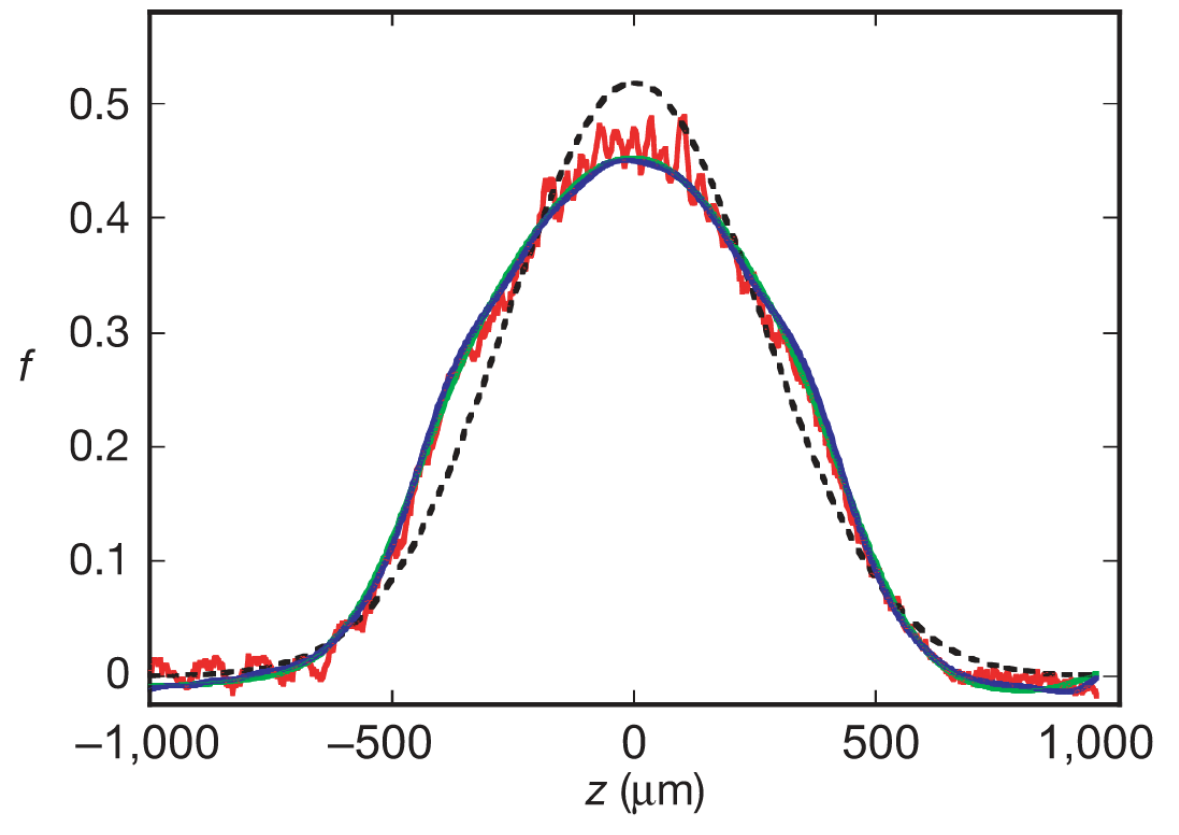
\includegraphics[width=1.0\textwidth]{dephased_momentum_distribution}
    \end{center}
    \caption{\label{dephased_momentum_distribution}
             The blue and green curves in the above figure are projections from
             models that take into account loss and heating. The red line is the
             actual distribution observed. The dashed line is a gaussian with
             the same number of atoms and r.m.s. width as the actual
             distribution.}
 \end{figure}


To the extent that the actual distribution in figure
\ref{dephased_momentum_distribution} conforms to the projected distribution
rather than to the gaussian, the atoms have not thermalised.

These observations extended from the Tonks--Girardeau regime, which has very
strong repulsive interactions between bosons so only pairwise collisions can
occur, to the intermediate coupling regime, where there can be three-
(or more) body collisions.


\subsection{Relaxation in a Completely Integrable Many-Body Quantum System}

Inspired by the ``A Quantum Newton's Cradle'' study, investigations were made
into a completely integrable many-body quantum system. In this experiment,
hard-core bosons on a one-dimensional lattice were used. The authors, Rigol et. al
\cite{Rigol2007}, started with a one-dimensional bosonic Hamiltonian with no
interactions and periodic boundary conditions for a lattice with $L$ lattice
sites.
\begin{equation}
 \hat{H}=-J\sum_{i=1}^{L} (\hat{a}_{i}^{\dagger}\hat{a}_{i+1}+h.c.)
\end{equation}

They then mapped their bosonic system to a free ferminonic one using a
Jordan-Wigner transformation:
\begin{equation}
 \hat{H}=-J\sum_{i=1}^{L} (\hat{c}_{i}^{\dagger}\hat{c}_{i+1}+h.c.)
\end{equation}
Here $\hat{c}_{i}^{\dagger}$ and $\hat{c}_{i+1}$ are fermionic creation and
annihilation operators. The integrals of motion were the fermionic
quasi-momentum distribution operators, and the system thus must be
integrable because there are as many of these operators as they had lattice
sites. They have numerically investigated the time evolution of this system and
found it to undergo relaxation to an equilibrium state. The properties of the
state that the system relaxed to were not given by the grand-canonical
ensemble, but rather by a generalised Gibbs ensemble, in which the partition
function is extended to include all of the integrals of motion.


\begin{figure}[H]
    \begin{center}
        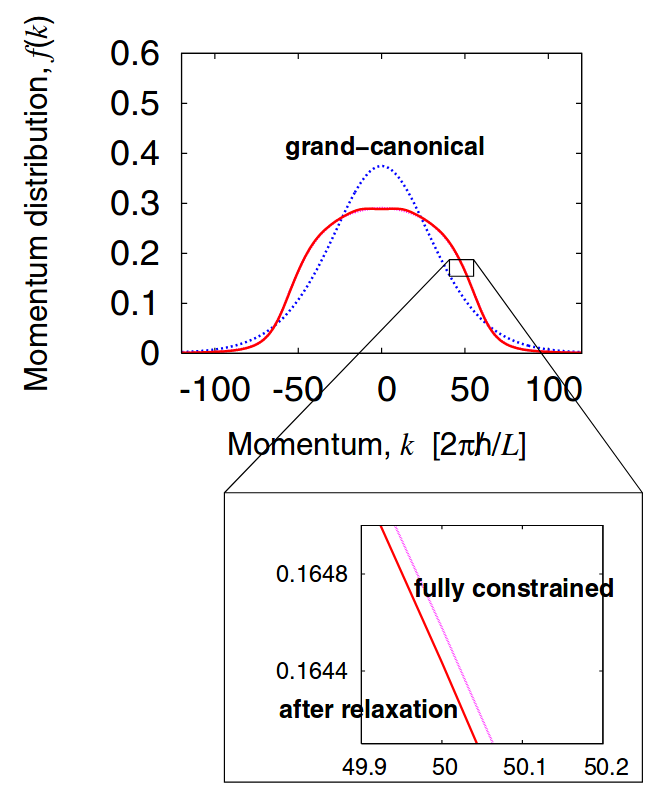
\includegraphics[width=8cm]{grand_canonical_vs_GGE}
    \end{center}
    \caption{Equilibrium (quasi-)momentum distribution after relaxation in
             comparison with the predictions of the grand-canonical and of the
             fully constrained thermodynamic ensembles. The prediction  of the
             fully constrained  ensemble  is virtually  indistinct from the
             results of the dynamical simulation. Image taken from
             \cite{Rigol2007}.}
 \end{figure}



They further showed that their generalised equilibrium state carries more memory
of the initial conditions than the usual thermodynamic one.
\begin{figure}[H]
    \begin{center}
        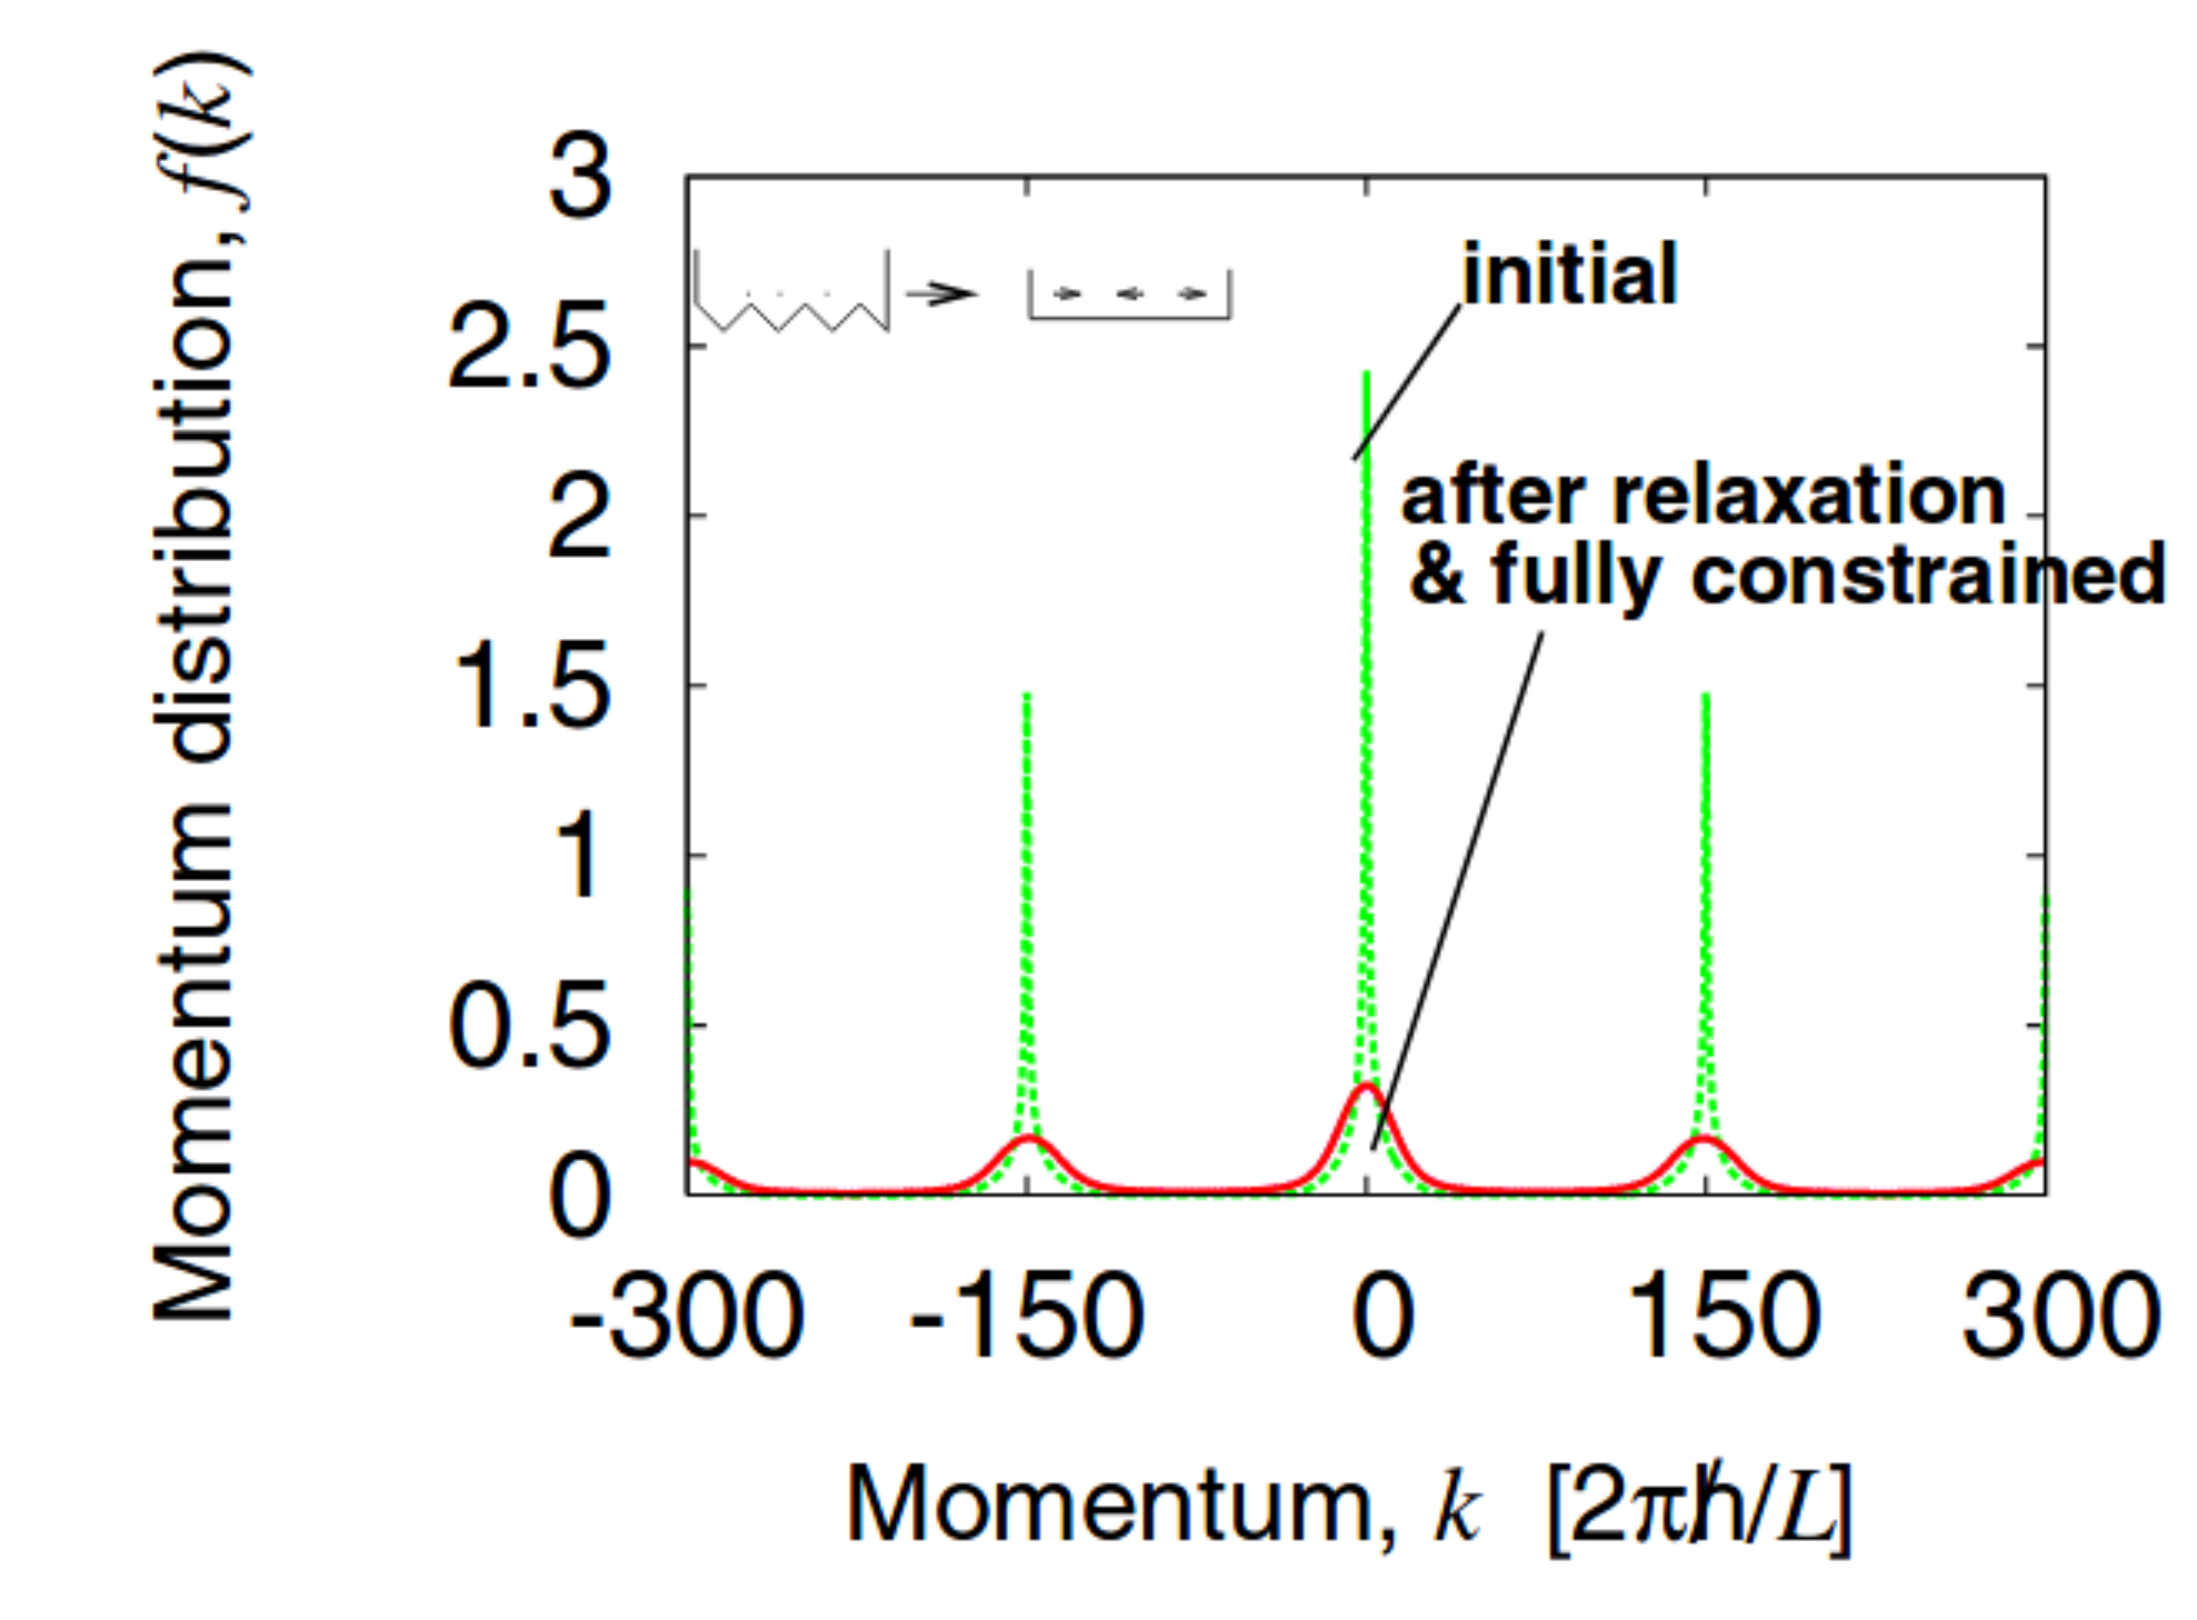
\includegraphics[width=8cm]{after_relaxation_rigol}
    \end{center}
    \caption{The actual quasi-momentum distribution after relaxation versus
             predictions of the generalised Gibbs ensemble and the grand
             canonical ensemble. Image taken from \cite{Rigol2007}.}
 \end{figure}

The momentum peaks remain clear and distinct during the whole duration  of
propagation; $t_{\text{fin}} = 3000 \hbar/J$.

\subsection{Measuring entanglement entropy in a quantum many-body system}

- I still don't see how this is supposed to relate to what I'm doing.
I can write down the definition of the nth order R\'enyi entropies, and
describe what purity is. I imagine that I could construct a system that is a
$2 \times N$ lattice and split it into two one-dimensional lattices of length N,
then evaluate their purity (which must be zero for one of the chains and 1 for
the other if I'm starting with all bosons on one site, right?), then do some
second order renyi entropy calculation based on that. Then I could evolve the
system in time and note that this entropy changes. How does that relate to
thermalisation? What can I find out from this approach that I don't already
get from just looking at expectation values of number operators?

\newpage

\section{System size and analyticity}

Whilst the main focus of this project is on smaller lattices with few
particles, it is of interest to investigate larger system sizes (necessarily
by approximate methods) to see how much of the behaviour of the small systems
is preserved in the larger ones.


\subsection{Small systems}

We can decompose any time evolved state $\ket{\psi(t)}$ of our system in terms
of its state at $t=0$, $\ket{\psi(0)}$, and the energy eigenvectors $\ket{E_n}$
(see section \ref{revival} for details):
\begin{equation}
    \ket{\psi(t)} = \sum_{j}{e^{i E_{j}t} \ket{E_{j}} \braket{E_{j}|\psi(0)}}.
\end{equation}
Calculating $\ket{\psi(t)}$ from the above formula requires that we diagonalise
the Hamiltonian and find its energy eigenvectors and eigenvalues. This is easy
for small systems, in particular those that have only a single particle on them.
This method has the significant advantage of being ``analytic'', at least up to
the precision of the values stored for the eigenvalues and eigenvectors. All
instances of $\ket{\psi(t)}$ are calculated from the initial state
$\ket{\psi(0)}$, so the value we calculate for $\ket{\psi(t)}$ is independent of the time-step
between each instance of $\ket{\psi(t)}$ that we calculate. This has the further
advantage that in a numerical algorithm we need not concern ourselves with
drifting of the norm. However, as the number of lattice
sites and particles in the system increases, the time required to apply this
method increases dramatically. This is because the dimensionality $\mathcal{D}$
of the system grows according to
\begin{equation}
    \label{dimensionality_exact}
    \mathcal{D} = \frac{(N + P - 1)!}{P! (N-1)!},
\end{equation}
where $N$ is the number of lattice sites and $P$ is the number of particles on
the lattice. Unsurprisingly, this is the same as the number of possible pure
number states (since these form an orthonormal basis), and so the formula
deduced is just the formula for the number of ways to arrange $P$ objects into
$N$ containers that is familiar from elementary statistical mechanics.
The Hamiltonian is a $\mathcal{D}\times\mathcal{D}$ square matrix, and
diagonalising it and then evolving the system according to equation
(\ref{dimensionality_exact}) quickly becomes impractical for systems with large
numbers of particles and lattice sites. We can use another familiar tool from
elementary statistical mechanics -- Stirling's approximation -- to clarify the
rate of growth of the dimensionality of the system. Stirling's
approximation \cite{Schroeder2007} is
\begin{equation}
    N! \approx N^{N} e^{-N} \sqrt{2 \pi N}.
\end{equation}
All of the following assumptions (including Stirling's approximation) are
valid only for large $N$.
\begin{equation*}
    \mathcal{D} = \frac{(N + P - 1)!}{P! (N-1)!}
    \approx
    \frac{(N + P)!}{P! N!}
\end{equation*}
Now applying Stirling's approximation to each factorial:
\begin{equation*}
    \mathcal{D}
    \approx
    \frac{(P + N)^{P+N} e^{-(P + N)} \sqrt{2 \pi (P+N)}}
         {P^{P} e^{-P} N^{N} e^{-N} 2 \pi \sqrt{PN}}
    =
    \frac{(P + N)^{P+N} \sqrt{2 \pi (P+N)}}
         {P^{P} N^{N} 2\pi \sqrt{PN}}.
\end{equation*}
The exponentials are much more significant than the multiplicative factors,
so we have
\begin{equation*}
    \mathcal{D} \approx \frac{(P + N)^{P+N}}{P^P N^N}.
\end{equation*}
In order to get a more concrete idea of how quickly the dimensionality of a
typical system would grow, consider the case where we have roughly one boson
per lattice site ($N \approx P$). In this case,
\begin{equation*}
    \mathcal{D} \approx \frac{(2P)^{2P}}{P^{P} P^{P}} = 2^{2P} = 4^{P}.
\end{equation*}
This means that when we increase the size of the system by one lattice site
with one boson on it, the dimensionality roughly quadruples. In light of
this exponential increase in dimensionality for large systems, a different
approach to time evolution is required. We have chosen to use a
Gross-Pitaevskii equation to reduce the dimensionality of the system. Doing
this forces us to take an iterative approach to time evolution rather than an
analytic one. A Runge-Kutta-Feldberg algorithm \cite{Burden2005} was written
for this purpose.


\subsection{The Gross-Pitaevskii Equation}

The Gross-Pitaevskii Equation (GPE) is a classical mean-field equation for
describing Bose-Einstein condensates (BECs) in the zero-temperature limit. In
the smaller systems that we consider with the analytic method, it is rare for us
to have more than two particles on a lattice, and hence the concept of
``macroscopic occupation of the ground state'' that is integral to Bose-Einstein
condensation has little importance here.

The validity of some of the assumptions that we make in this
method will rely on there being a large number of particles. When second
quantising our Hamiltonian earlier, in equation (\ref{field_operators_wannier})
we decomposed the field operators into linear combinations of single-particle
Wannier position states. However, it is possible to decompose the field
operators into any complete single-particle basis. If we chose the single
particle energy basis $\{\phi_i\}$, then we get
\begin{equation}
    \hat{\Psi}(\mathbf{r})
    =
    \sum_{i=0}^{\infty}{\hat{a}_i\phi_{i}(\mathbf{r})}
    =
    \hat{a}_{0} \phi_{0}(\mathbf{r}) +
    \sum_{i=1}^{\infty}{\hat{a}_i\phi_{i}(\mathbf{r})}.
\end{equation}
Since the GPE is a tool for investigating near-zero temperature BECs (very low
energy systems), we now assume that the occupancy of energy modes other than
the ground modes is negligible, i.e.,
\begin{equation}
 \hat{\Psi}(\mathbf{r})=\hat{a}_0\phi_{0}(\mathbf{r}).
\end{equation}
Next we note that when there are a large number of particles in the ground
state $\ket{N_0}$ then the action of the creation and destruction operators
on the ground state approximately commute:
\begin{equation}
 \hat{a}_0\hat{a}^\dagger_0\ket{N_0}
 =
 N_0 \sqrt{1+\frac{1}{N_0}}\ket{N_0}
 \approx
 N_0\ket{N_0}
 =
 \hat{a}^\dagger_0\hat{a}_0\ket{N_0}
\end{equation}
It is this property of commutation that leads us to replace the creation and
annihilation operators by $\sqrt{N_0}$, which allows us to approximate the
field operator $\hat{Psi}(\mathbf{r})$ with a wave function
\begin{equation}
    \hat{\Psi}(\mathbf{r})
    =
    \hat{a}_{0} \phi_{0}(\mathbf{r}) \approx N_{0} \phi_{0}(\mathbf{r})
    =
    \psi_{0}(\mathbf{r}).
\end{equation}

\subsection{Runge-Kutta-Feldberg Method}
The nonlinear term in the GPE prevents us from being able to represent the 
Hamiltonian in matrix form. Hence we cannot find the eigenvectors and 
eigenvalues of the system directly, which prevents us from using the 'analytic' 
approach to time evolution that we used for smaller system sizes. One method
that we could use in its pace is to simply expand the time evolution
operator $e^{-i\hat{H}t}$ in a Taylor series, truncated at an appropriate order,
i.e.,
\begin{equation}
 \ket{\psi(t)}
 =
 e^{-i\hat{H}t}\ket{\psi(0)}
 =
 \left
 (1
 +
 (-i\hat{H}t)
 +
 \frac{1}{2}(-i\hat{H}t)^2
 +
 \frac{1}{6}((-i\hat{H}t)^3
 +
 \dots
 \right)
 \ket{\psi(0)}.
\end{equation}
When we are working with systems in which $U_0 \neq 0$, the nonlinearity 
that is present quickly causes inaccuracies in any low-order ($\leq3$) Taylor 
method. This can be observed by calculating the norm of $\ket{\psi(t)}$ at 
each timestep (it quickly grows significantly greater than $1$). Using a 
higher-order Taylor method is slow, due to the computation time required to 
calculate the derivatives of $e^{-i\hat{H}t}$ at each timestep\todo{check this
is exactly correct}. 

A standard Runge-Kutta method speeds up the calculation by avoiding calculating 
these derivatives while retaining high-order truncation error. One of the most 
frequently used Runge-Kutta methods is a fourth order method, which has 
truncation error of $\mathcal{O}(h^4)$, where $h$ is the size of the timestep.

For a given differential equation 
\begin{equation}
 y'=f(t,y)
\end{equation}
with initial condition $y(t=0)=\alpha$, we can approximate the value of $y$ at
$N$ successive times (each separated by timestep $h$) by $w$, where
\begin{align*}
 w_0&=\alpha \\
 k_1&=hf(t_i,w_i) \\
 k_2&=hf\left(t_i+\frac{h}{2}),w_i+\frac{1}{2}k_1\right) \\
 k_3&=hf\left(t_i+\frac{h}{2}),w_i+\frac{1}{2}k_2\right) \\
 k_4=hf(t_{i+1},w_i+k_3) \\
 w_{i+1}=w_i+\frac{1}{6}(k_1+2k_2+2k_3+k4) \\
 \end{align*}
for each $i=0,1,\dots,N-1$. Setting $y=\ket{\psi(t)}$, $w_0=\psi(t=0)$ and 
$f(t,y)=i\hat{H}$.

\todo{blarg. need to work through this again to get it right}


Even when using this method, we are concerned about the effect of the nonlinear 
term on our error. Hence we adopt a more sophisticated algorithm 
(the Runge-Kutta-Feldberg method). This method incorporates a estimate of the
truncation error and adapts the step size as it goes to ensure that the error
stays below a certain tolerance set by the user. 

Specifically, it uses a Runge-Kutta method of order five to estimate the 
local error in a Runge-Kutta method of order four. If the estimated error
is greater than the tolerance, then the timestep is shortened and the error is 
estimated again. The interested reader may refer to chapter $5$ of 
\emph{Numerical Analysis} by R. Burden and J. Faires \cite{Burden2005} for the 
precise details of the algorithm used.



\section{Results}

\section{Revival \label{revival}}

In a subset of the integrable systems considered, we observed regular instances
in which the system would return to the state in which it was initially
prepared (it ``revives''). To see why we might expect to see revival in
some cases, consider the initial state of the system $\ket{\psi(0)}$, which
evolves in time according to
\begin{equation}
 \ket{\psi(t)}=e^{i\hat{H}t}\ket{\psi(0)}.
\end{equation}
Now noting that we can use the completeness relation for the energy eigenstates
to expand the initial state in the energy basis, and incorporating the
$\hbar^{-1}$ into the time scale,
\begin{align}
\label{time_evolution}
 \ket{\psi(t)} &= e^{i\hat{H}t}\sum_j\ket{E_j}\braket{E_j|\psi(0)}  \nonumber \\
               &= \sum_je^{i\hat{H}t}\ket{E_j}\braket{E_j|\psi(0)}  \nonumber \\
               &= \sum_je^{iE_{j}t}\ket{E_j}\braket{E_j|\psi(0)}    \nonumber \\
               &= \sum_j c_{j}e^{iE_{j}t}\ket{E_j}
\end{align}

From here it can be seen that the only time dependence appears in the complex
exponentials, each of which is $2\pi$-periodic. If we can find some common
time $t_r$ such that $E_{j} t^*=2 \pi k_{j}$, where $k_{j} \in \mathbb{Z} $
for all $j$, we will recover the initial state exactly, i.e.,
$\ket{\psi(t^*)}=\ket{\psi(0)}$. The next section describes the conditions
necessary for the existence of the revival time.\\


\subsection{Exact revival}

We observe an exact and regular revival in precisely the cases in which the
eigenvalues are mutually rational, i.e. they are either all rational, or are all
rational when divided by the same irrational number.
\begin{definition}[Mutually rational set]
    We say that a set of eigenvalues are mutually rational if they are all
    rational when divided by a common real number.
\end{definition}

For example, the set of
hypothetical eigenvalues $\lbrace 0, \sqrt{2}, 2 \sqrt{2}, \frac{3 \sqrt{2}}{10}
\rbrace$ is mutually rational, whereas $\lbrace 0, \sqrt{2}, \sqrt{3}\rbrace$ is
not. In the case of mutually rational eigenvalues, we can write $E_{j} =
\frac{p_{j}}{q_{j}}$, where $p_{j}$, $q_{j} \in \mathbb{Z}$. The revival time is
then given by
\begin{equation}
\label{revival_time_formula}
 t^* = \frac{2\pi Q_{LCM}}{P_{HCF}},
\end{equation}

where $Q_{LCM}$ is the
lowest common multiple of $\lbrace eq_j\rbrace$ and $P_{HCF}$ is the highest
common factor of the $\lbrace p_j \rbrace$.

We are yet to find any systems with nonzero interparticle interaction that have
mutually rational eigenvalues. In one dimension, the only systems that we have
found that meet the criterion of mutually irrational eigenvalues are those with
fewer than $4$ lattice sites. In two dimensions, the only systems that exhibit
revival have three or fewer chains and three or fewer lattice sites on each 
chain (see section \ref{2Dsystems}).

To demonstrate this exact revival, consider a one-dimensional lattice with three
sites with a single boson and hopping constant $J$. The Hamiltonian for this
system is
\begin{equation}
    \hat{H}_{3\times1}
    =
    \begin{pmatrix}
         0 & -J &  0 \\
        -J &  0 & -J \\
         0 & -J &  0
    \end{pmatrix}.
\end{equation}
Diagonalising this matrix yields the eigenvalues $\lbrace -\sqrt{2}J, 0,
\sqrt{2}J \rbrace$. These are mutually rational (if we divide them all by
$\sqrt{2}J$ they are all rational). If we rescale the energies by $\sqrt{2}J$ by
absorbing that factor into the time scale, then we get eigenvalues $\{-1,0,1\}$.
We can see from the graph of the simulation below that this matches up with a
return to the initial state at times that are multiples of $2\pi$.
\begin{figure}[H]
    \centering
    \begin{gnuplot}[terminal=cairolatex, terminaloptions={lw 2}, scale=0.95]
        set xlabel "$\\displaystyle \\frac{t}{\\sqrt{2}J}$"
        set ylabel "$\\langle n_{1} \\rangle$"
        plot "./Data/20170912T164043_evolution_n.dat" u 1:4 w l lc 1 notitle
     \end{gnuplot}
     \vspace*{-5mm}
     \label{3by1_noninteract_revival}
     \caption{Revival for a system with $3$ lattice sites and a
     single boson.}
\end{figure}

The reason that there appear to be several revivals that our method ``misses''
is that states with different phases in the coefficients of the eigenvectors
can also produce $\langle n_{1} \rangle = 1$, whereas the revival time that is
calculated in our method corresponds to exact revival of the initial
wave function and not $\langle n_{1} \rangle \sim \norm{\psi(t)}^{2}$.


\subsection{Approximate revival}

The range of systems for which the eigenvalues are mutually rational is a small
one. All systems which have nonzero interparticle interactions have mutually
irrational eigenvalues. One of the most interesting results so far is that
even in the one-dimensional single particle case, if there are more than
three lattice sites, the eigenvalues will be irrational. We can demonstrate this
by considering a single chain of five sites with one boson. The Hamiltonian for
this system is
\begin{equation}
    \hat{H}_{5\times1}
    =
    \begin{pmatrix}
         0 & -J &  0 &  0 &  0 \\
        -J &  0 & -J &  0 &  0 \\
         0 & -J &  0 & -J &  0 \\
         0 &  0 & -J &  0 & -J \\
         0 &  0 &  0 & -J &  0
    \end{pmatrix}.
\end{equation}
The eigenvalues of this system are $\lbrace -\sqrt{3}J, -J, 0, J, \sqrt{3}J
\rbrace$. These are clearly not mutually rational, so we cannot find an exact
revival time for this system, despite the fact that it is fully
integrable \cite{Rigol2007}. Note that the eigenvalues of a system with $4$
lattice sites are also mutually irrational (they are
$\frac{J}{2}\lbrace -1-\sqrt{5}, 1+\sqrt{5},1-\sqrt{5},-1+\sqrt{5}\rbrace$)
but those for a system of $5$ lattice sites are more convenient to work with.

Running a simulation of this system of $5$ lattice sites where we
start a single boson off on the first site, we find that the probability of
finding the boson on the first site never quite reaches unity again.
\begin{figure}[H]
    \centering
    \begin{gnuplot}[terminal=cairolatex, terminaloptions={lw 2}, scale=0.95]
        set xlabel "$\\displaystyle \\frac{t}{J}$"
        set ylabel "$\\langle n_{1} \\rangle$"
        plot "./Data/5by1_T1e4.dat" u 1:6 w l lc 1 notitle
     \end{gnuplot}
     \vspace*{-5mm}
     \caption{Absence of exact revival for a system with $5$
     lattice sites and a single boson.}
\end{figure}

Judging the figure above by eye, it may appear that we have exact revival, but
this is not actually the case. If we look at how long it takes for the system to
get within $\epsilon$ of its initial state (i.e. $\norm{\ket{\psi(t)} -
\ket{\psi(0)}} < \epsilon$) we get the graph below. Note that $t^*$ denotes the
time at which the system got within a particular value of $\epsilon$ of the
initial state.
\begin{figure}[H]
 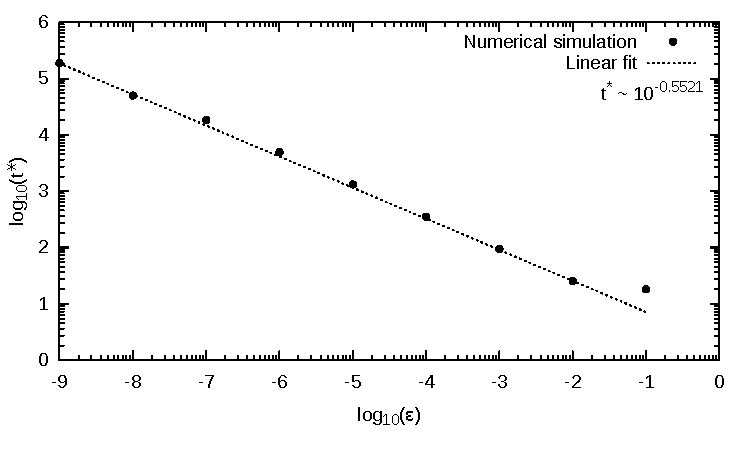
\includegraphics[width=1.0\textwidth]{recurrence_times}
 \centering
 \label{1Drecurrencetimes}
\end{figure}
While we see that the system does appear to get arbitrarily close to revival,
but it can take arbitrarily long to do so. This result can be explained in terms
of the Poincar\'e recurrence theorem.

\subsection{The Poincar\'e Recurrence Theorem}

In 1890, Henri Poincar\'e proved \todo{how to cite him?} the following theorem
for classical mechanics:
\begin{quote}
    Any phase-space configuration $(q, p)$ of a system enclosed in a finite
    volume will be repeated as accurately as one wishes after a finite (be it
    possibly very long) interval of time.
\end{quote}
This theorem was extended to quantum systems in 1956 by P. Bocchieri and A.
Loinger \cite{Bocchieri1957}, where they gave a slightly different form:

\begin{theorem*}[Quantum recurrence]
    Let us consider a system with discrete energy eigenvalues $E_{n}$; if
    $\Psi(t_{0})$ is its state vector in the Schr{\"o}dinger picture at the time
    $t_{0}$ and $\epsilon$ is any positive number, at least one time $t^*$ will
    exist such that the norm $\norm{\Psi(t^*) - \Psi(t_0)}$ of the vector $\Psi(t^*)
    - \Psi(t_{0})$ is smaller than $\epsilon$.
\end{theorem*}
\begin{proof}
    The proof presented by Bocchieri and Loinger shows the theorem to be true
    for an infinite-dimensional system. In this dissertation, we investigate
    only finite-dimensional systems, and a simpler version of the proof can be
    constructed. We first show that there is a time $t^{*}$ at which
    $\norm{\ket{\psi(t^{*})} - \ket{\psi(t_{0})}}^{2} < 2 \epsilon'$ for any
    $\epsilon' > 0$ and then extend this to $\norm{\ket{\psi(t^{*})} -
    \ket{\psi(t_{0})}} < \epsilon$. Note that in the following we will introduce
    the notation $\tau=t^{*} - t_0$ and $\alpha^{2}(t^{*}) = \norm{
    \ket{\psi(t^{*})} - \ket{\psi(t_{0})}}^{2}$.
    \begin{align*}
     \alpha^2(t^*)
     &= \left(\bra {\psi(t^*)}-\bra {\psi(t_0)}\right)
        \left(\ket{\psi(t^*)}-\ket{\psi(t_0)}\right)
     \\
     &= 2-\braket{\psi(t^*)|\psi(t_0)}-\braket{\psi(t_0)|\psi(t^*)}
     \\
     &= 2-\sum_{j,n=1}^{\mathcal{D}}c_n^* c_je^{iE_{n}t^*}e^{-iE_{j}t_{0}}
     \braket{E_n|E_j}
     -
     \sum_{j,n=1}^{\mathcal{D}}c_j^*c_ne^{iE_{j}t_{0}}e^{-iE_{n}t^*}
     \braket{E_j|E_n}
     \\
     &= 2
        -
        \sum_{n=1}^\mathcal{D} |c_n|^2 e^{iE_{n}(t^*-t_0)}
        -
        \sum_{n=1}^\mathcal{D} |c_n|^2 e^{-iE_{n}(t^*-t_0)}
        \qquad
        \text{since}
        \braket{E_j|E_n}
        =
        \delta_{ij}
     \\
     &=
     2 \sum_{n=1}^\mathcal{D} |c_n|^2\left(1-\cos\left(E_{n}\tau\right) \right)
     \qquad
     \text{because}
     \ \sum_{n=1}^\mathcal{D} |c_n|^2=1
     \\
     &\leq
     2\sum_{n=1}^\mathcal{D}\left(1-\cos\left(E_{n}\tau\right) \right).
    \end{align*}
    It is sufficient to show that there is a $\tau$ such that
    $\sum_{n=1}^{\mathcal{D}}{\left(1 - \cos{(E_{n}\tau)} \right)} < \epsilon'$.
    This is actually the case according to a standard result of the theory of
    the almost-periodic functions \cite{Besicovitch1954}.

    Evidently, if we know that there exists a time $t^{*}$ such that
    \begin{equation}
        \sum_{n=1}^{\mathcal{D}}%
            {\left ( 1 - \cos{\left(E_{n} \tau \right)} \right )}
        < \epsilon',
    \end{equation}
    then at this same time $\alpha^{2}(t^{*}) < 2 \epsilon'$, which implies
    \begin{equation*}
        \alpha(t^{*})
        =
        \norm{\ket{\psi(t^{*})} - \ket{\psi(t_{0})}} < \sqrt{2 \epsilon'}.
    \end{equation*}
    Taking $\epsilon = \sqrt{2 \epsilon'}$ shows that $\norm{\ket{\psi(t^{*})} -
    \ket{\psi(t_{0})}}$ is guaranteed be arbitrarily small at some arbitrarily
    large time $t^{*}$.
\end{proof}


\subsection{Large one-dimensional systems}

To determine the mutual rationality or mutual irrationality of the eigenvalues for
an arbitrarily large one-dimensional system with a single particle, we look to a
result about the eigenvalues of tridiagonal matrices proven by W. Yueh
\cite{Yueh2006}. A tridiagonal matrix has the form
\begin{equation}
    A_{N \times N}
    =
    \begin{pmatrix}
             b &      c &     0  &      0 &  \dots & 0 \\
             a &      b &     c  &      0 &  \dots & 0 \\
             0 &      a &     b  &      c &  \dots & 0 \\
             0 &      0 &     a  &      b &  \dots & 0 \\
        \vdots & \vdots & \vdots & \vdots & \ddots & c \\
             0 &      0 &     0  &      0 &      a & b
    \end{pmatrix}.
\end{equation}
It was shown that the eigenvalues of a matrix of this form are given by
\begin{equation}
\label{tridiagonal_eigenvalues_formula}
    \lambda_{k} = -b + 2 \sqrt{ac} \cos{\!\left( \frac{k \pi}{N+1} \right )}
\end{equation}
where $k=1$, 2,\dots, $N$. The Hamiltonian of any one-dimensional system with
$N$ sites and a single particle has exactly this form, namely
\begin{equation}
    \hat{H}_{N}
    =
    \begin{pmatrix}
         0 &     -J &     0  &      0 &  \dots &  0 \\
        -J &      0 &    -J  &      0 &  \dots &  0 \\
         0 &     -J &     0  &     -J &  \dots &  0 \\
         0 &      0 &    -J  &      0 &  \dots &  0 \\
    \vdots & \vdots & \vdots & \vdots & \ddots & -J \\
         0 &      0 &     0  &      0 &     -J &  0
    \end{pmatrix},
\end{equation}
and consequently has eigenvalues ($k=1$, 2, \dots, $N$.)
\begin{equation}
    \label{1D_eigenvalues}
    E_{k} = 2 J \cos{\!\left( \frac{k \pi}{N+1} \right)}.
\end{equation}
This result is particularly interesting when combined with Niven's theorem
\cite{DoubleIvan}.

\begin{theorem*}[Niven's theorem]
  If $\theta$ is rational in degrees, say $\theta=2\pi r$ for some rational
  number $r$, then the only rational values of the trigonometric functions of
  $\theta$ are as follows: $\sin \theta, \cos \theta =0, \pm\frac{1}{2},\pm1;\ \
  \sec\theta, \csc\theta=\pm1,\pm2; \\ \tan\theta,\cot\theta=0,\pm1.$
\end{theorem*}
In other words, this theorem tells us that if $x$ is rational \textit{in
degrees}, then the only possible rational values of $\cos(x)$ are $0, \pm
\frac{1}{2}$ and $\pm 1$. Note in our case that $\frac{k\pi}{N+1}\neq 0, \pi$
for $k=1$, 2, \dots, $N$, so $\cos{\!(\frac{k\pi}{N+1})} \neq \pm 1$ and we are
left with 3 rational options.

When we are evaluating in degrees, equation \eqref{1D_eigenvalues} becomes
\begin{equation}
    E_{k} = 2 J \cos{\!\left ( \frac{180k}{N+1} \right )}.
\end{equation}
The argument of cosine here is clearly rational since $N$ and $k$ are integers.
Hence we know that for a system with non-degenerate eigenvalues, there can be at
most three eigenvalues, $\lbrace 0, \pm \frac{J}{2} \rbrace$, that are rational. So
$\mathcal{D} \leq 3$ for a system with all eigenvalues rational (the lattice
must have at most 3 sites). We must have at least $(N-3)$ irrational eigenvalues
for any larger system size. 

The spectrum of a one-dimensional system with $N$ sites and a single particle
has proven to be \eqref{1D_eigenvalues}. It is apparent that $E_{k}$ is a
strictly monotonically decreasing function as $k$ increases because $\cos(x)$ is
strictly monotonically decreasing on the interval $x\in(0,\pi)$ and 
$0<\frac{k\pi}{N+1}<\pi$ for $k=1,\dots,N$. Thus, $E_{k_{2}} <
E_{k_{1}}$ whenever $k_{1} < k_{2}$. We have shown --invoking Niven's
theorem-- that for all $N>3$ the values of the cosine function are irrational.
However, this result on its own does not guarantee the violation of recurrence,
as the latter notion requires the energy eigenvalues to be {\emph{mutually}}
irrational. We thus have to prove that there is no such case when all
eigenvalues are the multiples of the same irrational number.

Below we answer the question: is there a {\emph{rational}} $\gamma$ such
that $E_{k_{1}} = \gamma E_{k_{2}}$ for $k_{1} \ne k_{2}$? 

\begin{theorem*}[Mutual Rationality Recurrence Theorem]
    Consider the sequence of energy eigenvalues
    \begin{equation*}
        E_{k} = \cos{\!\left ( \frac{k \pi}{N+1} \right )}
        \qquad k=1, 2, \dots N,
    \end{equation*}
    where $N >3$. There are no pair of integers, $k_{1}$ and $k_{2}$, and
    rational number $\gamma$ such the equality $E_{k_{1}} = \gamma E_{k_{2}}$ is
    satisfied.
\end{theorem*}
\begin{proof}
    First we notice that if the equality $E_{k_{1}} = \gamma E_{k_{2}}$ is
    satisfied for a particular triplet $(k_{1}, k_{2}, \gamma)$ with a rational
    $\gamma$, then swapping the indices and taking the reciprocal of $\gamma$
    also leads to a satisfactory triplet, $(k_{2}, k_{1}, \frac{1}{\gamma})$.
    Thus the rationality of $\gamma$ does not depend on whether $k_{1}$ is
    bigger than $k_{2}$ or the other way around.

    Without restricting generality we may assume that $k_{1} < k_{2}$. Therefore
    $E_{k_{1}} > E_{k_{2}}$ and consequently $\abs{\gamma} > 1$. Let us
    substitute the explicit expression of the spectrum in the equation
    \begin{align*}
        E_{k_{1}}
        &=
        \gamma E_{k_{2}}
        \\
        2 J \cos{\!\left ( \frac{k_{1} \pi}{N+1} \right )}
        &=
        2 J \cos{\!\left ( \frac{k_{2} \pi}{N+1} \right )}.
    \end{align*}
    This equation can be simplified by dividing both sides by $2J$, and using
    Euler's complex exponential expression for the trigonometric functions:
    \begin{equation*}
        \exp{\!\left ( i \,\frac{k_{1} \pi}{N+1} \right )}
        =
        \gamma \exp{\!\left ( i\,\frac{k_{2} \pi}{N+1} \right )}.
    \end{equation*}
    We have to keep in mind though that we only demand the equality of the real
    parts. Since there is no such $k$ value that $\cos{\!\bigl(\frac{k}{N+1}
\,\pi \bigr)}=
    0$, we may divide both sides of the equation above with the exponential on
    the right hand side:
    \begin{equation*}
        \exp{\!\left ( i\,\frac{k_{1}-k_{2}}{N+1} \,\pi\right )} = \gamma.
    \end{equation*}
    Raising both sides to the power of $(N+1)$ leads us to
    \begin{equation}
        \label{eq:NiksTheoremTranscendentalVsRational}
        e^{i (k_{1}-k_{2}) \pi} = \gamma^{N+1}.
    \end{equation}
    Notice that $e^{i (k_{1}-k_{2}) \pi} = (e^{i\pi})^{(k_{1}-k_{2}) } =
    (-1)^{k_{1}-k_{2}}$. Since both $k_{1}$ and $k_{2}$ are integers their
    difference is also an integer number, thus the left hand side of
    \eqref{eq:NiksTheoremTranscendentalVsRational} is $\pm 1$ depending on the
    parity of $(k_{1}-k_{2})$. Meanwhile the right hand side of
    \eqref{eq:NiksTheoremTranscendentalVsRational} is $\gamma^{N+1}$, where
    $\abs{\gamma} > 1$, therefore $\abs{\gamma^{N+1}} > 1$. Consequently this
    equation cannot have a solution triplet $(k_{1}, k_{2}, \gamma)$, where
    $k_{1}$, $k_{2}$ are integers between 1 and $N$ inclusively and $\gamma$ is
    rational.
\end{proof}
Hence, we have shown that all one-dimensional noninteracting systems with more
than three lattice sites should not exhibit recurrence, and are thus expected
to thermalise.

\subsection{Interacting one-dimensional systems}
\todo{Should I talk about dimensionality of Hamiltonian and/or having to choose
a numbering convention for the representation?}
Adding multiple interacting particles introduces a number of interesting 
features in the thermalisation properties of our system. We have found that
when weak interactions are present, thermalisation appears to occur in all 
one-dimensional systems, including those that exhibited clear and regular 
revival in the noninteracting case. We also note that with weak
interactions the long-term average for the expectation value of the number 
operators all tend towards $\frac{P}{N}$, i.e., the particles become evenly 
distributed on the lattice.\todo{confirm this happens the same way for lots
of different initial conditions.}
With stronger interactions, however, we observe localisation, which we will 
investigate in section \ref{changing_interaction_strength}. 

To see why the systems that exhibited revival in the noninteracting case 
thermalise once interactions are added, we consider the specific case of 
two bosons on a $3\times1$ lattice. In the absence of interactions, this 
is identical to a single boson on a $3\times1$ lattice, up to normalisation.
We can see from figure \ref{3by1_noninteract_revival} that we have exact revival
in this system. Once we have multiple particles with interactions in the system,
we need a larger dimensional basis to represent all of the distinct number 
states, and thus we need a larger Hamiltonian. We need to pick an ordering 
convention for our number states in order to define the representation of 
the Hamiltonian matrix. In this project, we have chosen to order the states
in such a way that the states with the lowest index have the most particles on
one particular side of the lattice, i.e.,
\begin{equation}
\ket{200}=\ket{1}, 
\ket{110}=\ket{2}, 
\ket{101}=\ket{3}, 
\ket{020}=\ket{4}, 
\dots, 
\ket{002}=\ket{10}.
\end{equation}

Using this basis, we can represent the Hamiltonian as

\begin{equation}
    \hat{H}_{3\times1}^{\left(P=2\right)}
    =
    \begin{pmatrix}
         U & -\sqrt{2}J & 0 & 0 & 0 & 0 \\
	-\sqrt{2}J & 0 & -\sqrt{2}J &  -J & 0 & 0 \\
	0 & -\sqrt{2}J & U &  0 & -\sqrt{2}J & 0 \\
	0 & -J & 0 & 0 & -J & 0\\0 & 0 & -\sqrt{2}J & -J & 0 & -\sqrt{2}J \\ 
	0 & 0 & 0 & 0 & -\sqrt{2}J & U
    \end{pmatrix}.
\end{equation}

The eigenvalues of this system are
\begin{align*}
 \lambda_1&=U_0 \\ 
 \lambda_2&= \frac{1}{2}\left(U_0 - \sqrt{8J^2 + U_0^2}\right)\\ 
 \lambda_3&=\frac{1}{2}(U_0 + \sqrt{8J^2 + U_0^2})\\
 \lambda_4&=\frac{U_0}{3} - \frac{-24J^2 - U_0^2}{{3\left(9J^2U_0 + U_0^3 + 3\sqrt{3}\sqrt{-512J^6 - 61J^4U_0^2 - 2J^2U_0^4}}\right)^{\frac{1}{3}}} \\ 
 &+ \frac{1}{3}(9J^2U_0 + U_0^3 + 3\sqrt{3}
    \sqrt{-512J^6 - 61J^4U_0^2 - 2J^2U_0^4})^{\frac{1}{3}}\\
 \lambda_5&= \frac{U_0}{3} + 
 \frac{(1 + i\sqrt{3})(-24J^2 - U_0^2)}{{6\left(9J^2U_0 + U_0^3 + 3\sqrt{3}\sqrt{-512J^6 - 61J^4U_0^2 - 2J^2U_0^4}}\right)
   ^{\frac{1}{3}}}\\
   &-\frac{1}{6}(1 - i\sqrt{3})
   \left(9J^2U_0 + U_0^3 + 3\sqrt{3}\sqrt{-512J^6 - 61J^4U_0^2 - 2J^2U_0^4}\right)^{\frac{1}{3}}\\
 \lambda_6&= \frac{U_0}{3} + \frac{(1 - i\sqrt{3})(-24J^2 - U_0^2)}{{6\left(9J^2U_0 + U_0^3 + 3\sqrt{3}\sqrt{-512J^6 - 61J^4U_0^2 - 2J^2U_0^4}\right)^
   {\frac{1}{3}}}}\\
   &- \frac{1}{6}(1 + i\sqrt{3})
   \left(9J^2U_0 + U_0^3 + 3\sqrt{3}\sqrt{-512J^6 - 61J^4U_0^2 - 2J^2U_0^4}\right)^{\frac{1}{3}}
\end{align*}
There are some eigenvalues in the above set with multiplicity greater than one.
Whilst we have not proven that the above eigenvalues form a mutually irrational
set, when we consider the number of square roots and third roots in the above
set of eigenvalues, we see that it at least appears very unlikely that a 
particular combination of $J$ and $U_0$ would result in a mutually rational
set of eigenvalues. 

When we run a simulation of this system, we find that the long term average
for the particle to be on the same site that it started on approaches 
$\frac{P}{N}=\frac{2}{3}$, which is consistent with it thermalising.

\begin{figure}[H]
    \centering
    \begin{gnuplot}[terminal=cairolatex, terminaloptions={lw 2}, scale=0.95]
        f(x)=0.667
        g(x)=0.70387
        P(x)=2
	set yrange [0:2.5]
        set xlabel "$\\displaystyle \\frac{t}{\\sqrt{2}J}$"
        set ylabel "$\\langle n_{1} \\rangle$"
        plot "./Data/3by1_U0.1_T2e4.dat" u 1:4 w l lc 1 notitle, f(x) title "$P/N=0.67$" w l, g(x) title "$\\overline{\\langle n_{1} \\rangle}$" w l, P(x) title "$P=2$"
     \end{gnuplot}
     \vspace*{-5mm}
     \caption{Thermalisation for a $3\times 1$ lattice
     with two bosons and $U=0.1$.}
\end{figure}

We observe something similar in the case of a $2\times1$ lattice with two 
bosons on it. Here we expect the long term average to be $\frac{P}{N}=
\frac{2}{2}=1$, which is consistent with what we see.
\todo{on reflection, this looks a bit like revival. Look at data file to test.}

\begin{figure}[H]
    \centering
    \begin{gnuplot}[terminal=cairolatex, terminaloptions={lw 2}, scale=0.95]
	f(x)=1
	g(x)=1.0066
	P(x)=2
	set yrange [0:2.5]
        set xlabel "$\\displaystyle \\frac{t}{\\sqrt{2}J}$"
        set ylabel "$\\langle n_{1} \\rangle$"
        plot "./Data/2by1_U0.1_T1e4.dat" u 1:3 w l lc 1 notitle, f(x) title "$P/N=1$" w l, g(x) title "$\\overline{\\langle n_{1} \\rangle}$" w l, P(x) title "$P=2$"
     \end{gnuplot}
     \vspace*{-5mm}
     \caption{Thermalisation for a $2\times 1$ lattice
     with two bosons and $U_0=0.1$.}
\end{figure}

We see a similar pattern with a $3\times1$ lattice with two particles, with the
long-term average being $2/3$.
 
The agreement of the long-term average with a uniform spatial distribution is
also clear for larger system sizes, such as a $10\times1$ lattice with
two bosons, as demonstrated in figure (\ref{10by1_U0.1}), where $\frac{P}{N}
=0.2$.
\begin{figure}[H]
    \centering
    \begin{gnuplot}[terminal=cairolatex, terminaloptions={lw 2}, scale=0.95]
        f(x)=0.2
        g(x)=0.24110
        P(x)=2
	set yrange [0:2.5]
        set xlabel "$\\displaystyle \\frac{t}{\\sqrt{2}J}$"
        set ylabel "$\\langle n_{1} \\rangle$"
        plot "./Data/10by1_U0.1_T2e4.dat" u 1:11 w l lc 1 notitle, f(x) title "$P/N=0.2$" w l, g(x) title "$\\overline{\\langle n_{1} \\rangle}$" w l, P(x) title "$P=2$"
     \end{gnuplot}
     \vspace*{-5mm}
     \caption{Thermalisation for a $10\times 1$ lattice
     with two bosons and $U=0.1$.}
     \label{10by1_U0.1}
\end{figure}

\subsubsection{Effect of interaction 
strength\label{changing_interaction_strength}}

When the interaction strength is increased, we notice an increasing 
dependence of the long-term averages of the expectation values of the number 
operators. This suggests that having strong interparticle interactions can 
frustrate thermalisation. \todo{add more words here}
All of the following simulations are run for a $3\times1$ lattice with two
bosons. U=0.005 (short term)

\begin{figure}[H]
    \centering
    \begin{gnuplot}[terminal=cairolatex, terminaloptions={lw 2}, scale=0.95]
	f(x)=0.6667
	g(x)=0.70245
	P(x)=2
	set yrange [0:2.5]
        set xlabel "$\\displaystyle \\frac{t}{J}$"
        set ylabel "$\\langle n_{1} \\rangle$"
        plot "./Data/3by1_U0.005_T2e4.dat" u 1:4 w l lc 1 notitle, f(x) title "$P/N=0.67$" w l, g(x) title "$\\overline{\\langle n_{1} \\rangle}$" w l, P(x) title "$P=2$" 
     \end{gnuplot}
     \vspace*{-5mm}
     \caption{Demonstrating thermalisation for a $3\times 1$ lattice
     with two bosons and $U=0.005$. The long time average of 
     $\langle n_1 \rangle$ is $\overline{\langle n_1 \rangle}=0.70245.$}
\end{figure}

The time average of the expectation value of the number operator
for the first site, $\overline{\langle n_1 \rangle}=0.70245.$, is 
greater than $\frac{P}{N}=0.67$. This may appear to be a result of the 
contributions to the time average of the early timesteps, as the bosons were
on the first site at t=0. However, running a simulation with the same 
parameters for $5$ times as long gives an average that is nearly 
indistinguishable from this, suggesting that the early data is not skewing the
result.\\
U=0.005 (long term)

\begin{figure}[H]
    \centering
    \begin{gnuplot}[terminal=cairolatex, terminaloptions={lw 2}, scale=0.95]
	f(x)=0.6667
	g(x)=0.70280
	P(x)=2
	set yrange [0:2.5]
        set xlabel "$\\displaystyle \\frac{t}{J}$"
        set ylabel "$\\langle n_{1} \\rangle$"
        plot "./Data/3by1_U0.005_T1e5.dat" u 1:4 w l lc 1 notitle, f(x) title "P/N=0.67" w l, g(x) title "$\\overline{\\langle n_{1} \\rangle}$" w l, P(x) title "$P=2$"
     \end{gnuplot}
     \vspace*{-5mm}
     \caption{Thermalisation for a $3\times 1$ lattice
     with two bosons and $U=0.005$. The long time average of 
     $\langle n_1 \rangle$ is $\overline{\langle n_1 \rangle}=0.70280.$}
\end{figure}

U=0.01


\begin{figure}[H]
    \centering
    \begin{gnuplot}[terminal=cairolatex, terminaloptions={lw 2}, scale=0.95]
	f(x)=0.6667
	g(x)=0.70329
	P(x)=2
	set yrange [0:2.5]
        set xlabel "$\\displaystyle \\frac{t}{J}$"
        set ylabel "$\\langle n_{1} \\rangle$"
        plot "./Data/3by1_U0.01_T1e5.dat" u 1:4 w l lc 1 notitle, f(x) title ``P/N=0.67'' w l, g(x) title "$\\overline{\\langle n_{1} \\rangle}$" w l, P(x) title "$P=2$"
     \end{gnuplot}
     \vspace*{-5mm}
     \caption{Thermalisation for a $3\times 1$ lattice
     with two bosons and $U_0=0.01$. The long time average of 
     $\langle n_1 \rangle$ is $\overline{\langle n_1 \rangle}=0.70329.$}
\end{figure}


U=0.01 (to T=1e6)

\begin{figure}[H]
    \centering
    \begin{gnuplot}[terminal=cairolatex, terminaloptions={lw 2}, scale=0.95]
        set title "Probability that boson found on first site over time"
	f(x)=0.6667
	g(x)=0.70319
	P(x)=2
	set yrange [0:2.5]
        set xlabel "$\\displaystyle \\frac{t}{J}$"
        set ylabel "$\\langle n_{1} \\rangle$"
        plot "./Data/3by1_U0.01_T1e6dt1.dat" u 1:4 w l lc 1 notitle, f(x) title "P/N=0.67" w l, g(x) title "$\\overline{\\langle n_{1} \\rangle}$" w l, P(x) title "$P=2$"
     \end{gnuplot}
     \vspace*{-5mm}
     \caption{Thermalisation for a $3\times 1$ lattice
     with two bosons and $U_0=0.01$. The long time average of 
     $\langle n_1 \rangle$ is $\overline{\langle n_1 \rangle}=0.70319.$}
\end{figure}

U=0.1 

\begin{figure}[H]
    \centering
    \begin{gnuplot}[terminal=cairolatex, terminaloptions={lw 2}, scale=0.95]
        f(x)=0.6667
        g(x)=0.70390
        P(x)=2
	set yrange [0:2.5]
        set xlabel "$\\displaystyle \\frac{t}{J}$"
        set ylabel "$\\langle n_{1} \\rangle$"
        plot "./Data/3by1_U0.1_T2e4.dat" u 1:4 w l lc 1 notitle, f(x) title "P/N=0.67" w l, g(x) title "$\\overline{\\langle n_{1} \\rangle}$" w l, P(x) title "$P=2$"
     \end{gnuplot}
     \vspace*{-5mm}
     \caption{Thermalisation for a $3\times 1$ lattice
     with two bosons and $U=0.1$. The long time average of 
     $\langle n_1 \rangle$ is $\overline{\langle n_1 \rangle}=0.70390.$}
\end{figure}

U=0.5

\begin{figure}[H]
    \centering
    \begin{gnuplot}[terminal=cairolatex, terminaloptions={lw 2}, scale=0.95]
        f(x)=0.6667
        g(x)=0.71241
        P(x)=2
	set yrange [0:2.5]
        set xlabel "$\\displaystyle \\frac{t}{J}$"
        set ylabel "$\\langle n_{1} \\rangle$"
        plot "./Data/3by1_U0.5_T2e4.dat" u 1:4 w l lc 1 notitle, f(x) title "P/N=0.67" w l, g(x) title "$\\overline{\\langle n_{1} \\rangle}$" w l, P(x) title "$P=2$"
     \end{gnuplot}
     \vspace*{-5mm}
     \caption{Thermalisation for a $3\times 1$ lattice
     with two bosons and $U_0=0.5$. The long time average of 
     $\langle n_1 \rangle$ is $\overline{\langle n_1 \rangle}=0.71241$.}
\end{figure}

U=2

\begin{figure}[H]
    \centering
    \begin{gnuplot}[terminal=cairolatex, terminaloptions={lw 2}, scale=0.95]
        P(x)=2
	set yrange [0:2.5]
        g(x)=0.77936
        f(x)=0.6667
        set xlabel "$\\displaystyle \\frac{t}{J}$"
        set ylabel "$\\langle n_{1} \\rangle$"
        plot "./Data/3by1_U2_T1e6dt1.dat" u 1:4 w l lc 1 notitle, f(x) title "P/N=0.67" w l, g(x) title "$\\overline{\\langle n_{1} \\rangle}$" w l, P(x) title "$P=2$"
     \end{gnuplot}
     \vspace*{-5mm}
     \caption{Thermalisation for a $3\times 1$ lattice
     with two bosons and $U_0=5$. The long time average of 
     $\langle n_1 \rangle$ is $\overline{\langle n_1 \rangle}=0.77936.$}
\end{figure}

U=5

\begin{figure}[H]
    \centering
    \begin{gnuplot}[terminal=cairolatex, terminaloptions={lw 2}, scale=0.95]
        P(x)=2
	set yrange [0:2.5]
        g(x)=0.88260
        f(x)=0.6667
        set xlabel "$\\displaystyle \\frac{t}{J}$"
        set ylabel "$\\langle n_{1} \\rangle$"
        plot "./Data/3by1_U5_T2e4.dat" u 1:4 w l lc 1 notitle, f(x) title "P/N=0.67" w l, g(x) title "$\\overline{\\langle n_{1} \\rangle}$" w l, P(x) title "$P=2$"
     \end{gnuplot}
     \vspace*{-5mm}
     \caption{Thermalisation for a $3\times 1$ lattice
     with two bosons and $U_0=5$. The long time average of 
     $\langle n_1 \rangle$ is $\overline{\langle n_1 \rangle}=0.88260.$}
\end{figure}

We can look at the long-term averages for the expecation value of the occupation
of all of the lattice sites (not just the one that the boson started on). When
we do this, a remarkable pattern emerges. If we start the boson on the first 
site, for low values of $U_0$ the average time spent on the second site is 
slightly lower than the outer lattice sites. We believe this to be a result of 
the repulsive contact interactions. However, once $U_0$ gets larger (especially
once it becomes greater than $1$), we find that the long-term average for
the site furthest from the one that the boson begins on drops dramatically.

\begin{figure}[H]
    \centering
    \begin{gnuplot}[terminal=cairolatex, terminaloptions={lw 2}, scale=0.95]
        set yrange [0:1]
        set xlabel "$U_0$"
        set ylabel "$Long term averages$"
        plot "./Data/Long_term_averages_for_3by1_systems" u 1:2 w l lc lp 1 title "$\\overline{\\langle n_{1} \\rangle}$", "./Data/Long_term_averages_for_3by1_systems" u 1:3 w l lp title "$\\overline{\\langle n_{2} \\rangle}$", "./Data/Long_term_averages_for_3by1_systems" u 1:4 w l lp title "$\\overline{\\langle n_{3} \\rangle}$"
     \end{gnuplot}
     \vspace*{-5mm}
     \label{3by1_comparisons}
     \caption{Long term averages for $3\times1$ systems with varying 
     interparticle interaction strengths}
\end{figure}

We have run simulations for higher values of $U_0$ in which we see that 
$\overline{\langle n_{1} \rangle}$ and $\overline{\langle n_{2} \rangle}$
asymptotically approach unity, and $\overline{\langle n_{3} \rangle}$ approaches
zero. 

One potential explanation for this behaviour is as follows. If the interparticle 
interactions are so powerful, beginning the system with both particles on
the same site means that the system has very high energy. When one of the 
particles moves to the second lattice site, conservation of energy demands
that the system still have high energy, but the interparticle interactions
only apply to bosons on the same site. Hence, the boson must gain a large 
amount of kinetic energy. The kinetic energy is proportional to the 
curvature of the wavefunction ($\sim \nabla^2\psi$), and hence the boson must be
highly localised within the second lattice site. The stronger the interparticle
interactions, the more kinetic energy this boson must have and thus the more
localised it is. This ``narrowness'' of the boson's spatial wavefunction \
reduces its tendency to tunnel into the third lattice site, so 
$\overline{\langle n_{3} \rangle}$ goes to zero. This behaviour suggests
that the system undergoes a quantum phase transition from a superfluid (when 
$U_0$ is small)to a Mott insulator (when $U_0$ is large).

This suggestion that what we are observing is a quantum phase transition is 
inspired by work done\todo{this is in their introduction, not their experiment. 
So is ``work done" the right terminology?} by Greiner et al. \cite{Greiner2002}, 
who state that for a system described by the Bose-Hubbard Hamiltonian

\begin{equation}
\begin{align*}
\hat{H}
=
&J\sum_{i}(\hat{a}^\dagger_{i}\hat{a}_{i+1}+h.c.\ )
+
\frac{U_0}{2}\sum_{i}\hat{a}^\dagger_{i}\hat{a}^\dagger_{i}
\hat{a}_{i}\hat{a}_{i},
\end{align*}
\end{equation}
in the limit where the tunneling term dominates the Hamiltonian, the 
ground-state energy is minimised if each of the single-particle wavefunctions of $P$
atoms are spread out over the entire lattice of $N$ lattice sites. This is
consistent with the values that we found for the long-term averages of number
operator expectation values for $U_0<<J$, which were close to $\frac{P}{N}$.

They further note that if system is homogeneous (i.e. 
$\epsilon_i=\text{const}$), as our systems are, then the many-body ground state
is given by

\begin{equation}
 \ket{\Psi_SF}^{\left(U_0=0\right)}
 \propto 
 \left( \sum_{i=1}^N \hat{a}_i^\dagger \right) ^P 
 \ket{0}.
\end{equation}

[This state is well described by a macroscopic wavefunction with long range 
phase coherence throughout the lattice]\todo{ask exactly what sentence in "[]" 
means, then reword}. 

On the other hand, if $U_0$ dominates the Hamiltonian\todo{maybe I can talk 
about Tonks-Girardeau gas somewhere in here, see highlighted paper}, then the 
ground state of the system is given by highly localised atomic wavefunctions
with a \emph{fixed number} of atoms per lattice site that minimise the 
interaction energy \cite{Bloch2005}. For a homogeneous lattice, this ground state is
\begin{equation}
 \ket{\Psi_MI}^{\left(J=0\right)}
 \propto 
  \prod_{i=1}^N \left( \hat{a}_i^\dagger \right)^\frac{P}{N} 
 \ket{0}.
\end{equation}
This state has very little phase coherence, but perfect correlations in particle
number exist between lattice sites\todo{see square brackets}. [does this mean 
that when P<N each lattice site has either one particle on it or zero? If so, 
then point out that this is consisten with the data in figure 
\ref{3by1_comparisons}]. The most important observation that we make about this 
Mott insulator state is that it cannot be described by a macroscopic
wavefunction, and so when we later use the Gross-Pitaevskii equation we will
not be able to legitimately consider systems with $U_0>J$.

\section{Two-dimensional systems\label{2Dsystems}}

\subsection{Single particle case}

In the single particle case (which is identical to the many-particle
non-interacting case, up to normalisation), the Hamiltonian is given by
\begin{equation}
    \hat{H}_{2D}
    =
    \left (
        J \sum_{i,j}{\hat{a}^{\dagger}_{i,j+1} \hat{a}_{i,j}} +
        J'\sum_{i,j}{\hat{a}^{\dagger}_{i,j}   \hat{a}_{i+1,j}}
    \right )
    +
    h.c.
\end{equation}
Like in the one-dimensional single-particle case, the Hamiltonian is an
$N \times N$ square matrix. We see many similarities between these systems
and one-dimensional single particle systems. We can attribute this to 
the fact that, in the absence of any interparticle interactions, the 
two-dimensional systems are separable. To demonstrate this, consider the Hamiltonian
for a $3\times3$ lattice with a single boson on it, with hopping in the 
$x$-direction characterised by $J$ and hopping in the $y$-direction 
characterised by $J'$ 

\begin{equation}
    \hat{H}_{3\times3}
    =
    \begin{pmatrix}
         0  & -J  &  0  & -J' &  0  &  0  &  0  &  0  &  0  \\
        -J  &  0  & -J  &  0  & -J' &  0  &  0  &  0  &  0  \\
         0  & -J  &  0  &  0  &  0  & -J' &  0  &  0  &  0  \\
        -J' &  0  &  0  &  0  & -J  &  0  & -J' &  0  &  0  \\
         0  & -J' &  0  & -J  &  0  & -J  &  0  & -J' &  0  \\
         0  &  0  & -J' &  0  & -J  &  0  &  0  &  0  & -J' \\
         0  &  0  &  0  & -J' &  0  &  0  &  0  & -J  &  0  \\
         0  &  0  &  0  &  0  & -J' &  0  & -J  &  0  & -J  \\
         0  &  0  &  0  &  0  &  0  & -J' &  0  & -J  &  0
    \end{pmatrix}.
\end{equation}

We use this example rather than a $2\times2$ lattice because the $2\times2$ 
lattice is not strictly two-dimensional (it is equivalent to a $4 \times1$ 
system with periodic boundary conditions). We note that this $3\times3$ system
can be considered as a combination of two $3\times1$ systems, one with hopping 
$J$ and the other with hopping $J'$, i.e.

\begin{equation}
 \hat{H}_{3\times3}=\hat{H}_{3\times1}^{(J)}\otimes {I}_3
 +
 {I}_3\otimes H_{3\times1}^{(J')},
\end{equation}
where 
\begin{equation}
    \hat{H}_{3\times1}^{(J)}
    =
    \begin{pmatrix}
         0 & -J &  0 \\
        -J &  0 & -J \\
         0 & -J &  0
    \end{pmatrix},
    \quad
    H_{3\times1}^{(J')}
    =
    \begin{pmatrix}
         0 & -J' &  0 \\
        -J' &  0 & -J' \\
         0 & -J' &  0
    \end{pmatrix},
\end{equation}
and $I_3$ is the $3\times3$ identity matrix, while $\otimes$ is a Kronecker 
tensor product.
Since the individual $3\times1$ systems exihibit revival, it is unsurpising that 
the two-dimensional one (almost always) does too. The revival time for the 
overall system is simply the lowest common multiple of the revival times of the
one-dimensional systems. Consequently, the case for which we do
not see revival in a $3\times3$ noninteracting system is when $J$ and $J'$ are
mutually irrational, as this renders their revival times mutually irrational 
\todo{Need to finish this argument off here, am too tired to do it atm}.

The separability of these \todo{quasi-two-dimensional}two-dimensional systems
suggests that if either of the systems that it separates into have mutually
irrational eigenvalues (and thus do not exhibit revival) then the whole system
will not revive either. In other words, if we have an $m\times n$ lattice, then
we will see thermalisation if $\text{max}\lbrace m,n \rbrace >3$.

We can now look at the simulation of several systems to demonstrate that
the above condition for revival or thermalisation holds.

Consider first the time evolution, figure \ref{3by3_equal_hop_U0}, of 
a boson that starts in the top left corner (``first lattice site'') of 
a $3 \times3$ lattice with $J=J'$.
\begin{figure}[H]
    \centering
    \begin{gnuplot}[terminal=cairolatex, terminaloptions={lw 2}, scale=0.95]
        set xlabel "$\\displaystyle \\frac{t}{\\sqrt{2}J}$"
        set ylabel "$\\langle n_{1} \\rangle$"
        plot "./Data/3by3T1e2H-2rescaled.dat" u 1:10 w l lc 1 notitle
     \end{gnuplot}
     \vspace*{-5mm}
     \caption{Revival for a $3 \times 3$ square lattice with a
     single boson and $J=J'$.}
     \label{3by3_equal_hop_U0}
\end{figure}

The \todo{should I get rid of this text}eigenvalues for this system (with $J=J'$) are
\begin{equation*}
    \lbrace 0, \pm\sqrt{2} J, \pm 2 \sqrt{2} J \rbrace
    \quad \text{or after scaling} \quad
    \lbrace 0,\pm 1,\pm 2 \rbrace.
\end{equation*}
These energy eigenvalues are clearly mutually rational. We also note that we
must have degeneracy in the eigenvalues now due to several symmetries of
geometric origin (e.g., rotation by $\frac{\pi}{2}$), which was not possible in
the one-dimensional case, as is clear from equation (\ref{1D_eigenvalues}).

Now consider a case identical to the previous one, except with $J=1$
and $J'=3/5$. Note that equation (\ref{revival_time_formula}) predicts
a revival time of $t^*=10\pi$ \todo{should $t^*$ be over $\sqrt{2}$?} here, which is
consistent with the simulation.

\begin{figure}[H]
    \centering
    \begin{gnuplot}[terminal=cairolatex, terminaloptions={lw 2}, scale=0.95]
        set xlabel "$\\displaystyle \\frac{t}{\\sqrt{2}}$"
        set ylabel "$\\langle n_{1} \\rangle$"
        plot "./Data/3by3T1e2H-2rescaledJP0.6.dat" u 1:10 w l lc 1 notitle
     \end{gnuplot}
     \vspace*{-5mm}
     \caption{Revival for a $3 \times 3$ square lattice with a
     single boson and $\lbrace J,J'\rbrace$ mutually rational.}
\end{figure}
If we now consider the case where $J$ and $J'$ are not mutually rational,
then we see that we do not get full revival, see figure 
\ref{3by1JJdashmutuallyirrational}.

\begin{figure}[H]
    \centering
    \begin{gnuplot}[terminal=cairolatex, terminaloptions={lw 2}, scale=0.95]
        set xlabel "$\\displaystyle \\frac{t}{\\sqrt{2}}$"
        set ylabel "$\\langle n_{1} \\rangle$"
        plot "./Data/3by3T1e3J1JP1_sqrt2.dat" u 1:10 w l lc 1 notitle
     \end{gnuplot}
     \vspace*{-5mm}
     \label{3by1JJdashmutuallyirrational}
     \caption{Absence of revival for a $3\times 3$ lattice
     with a single boson and $\lbrace J,J'\rbrace$ mutually 
     irrational: $J=1$ and $J'=\frac{1}{\sqrt{2}}$}
\end{figure}

The principles discussed earlier lead us to expect revival to be absent from
$4\times4$ systems, such as the following one with $J=J'$.

\begin{figure}[H]
    \centering
    \begin{gnuplot}[terminal=cairolatex, terminaloptions={lw 2}, scale=0.95]
        set xlabel "$\\displaystyle \\frac{t}{\\sqrt{2}J}$"
        set ylabel "$\\langle n_{1} \\rangle$"
        plot "./Data/4by4T1e3.dat" u 1:17 w l lc 1 notitle
     \end{gnuplot}
     \vspace*{-5mm}
     \caption{Absence of revival for a $4\times4$ lattice
     with a single boson and $J=J'$.}
\end{figure}

Is it worth putting in a larger system, like the following one?
$15\times15$ with $J=J'$.

\begin{figure}[H]
    \centering
    \begin{gnuplot}[terminal=cairolatex, terminaloptions={lw 2}, scale=0.95]
        set xlabel "$\\displaystyle \\frac{t}{J}$"
        set ylabel "$\\langle n_{1} \\rangle$"
        plot "./Data/15by15T1e3notscaled.dat" u 1:226 w l lc 1 notitle
     \end{gnuplot}
     \vspace*{-5mm}
     \caption{Absence of revival for a $15 \times 15$ lattice
     with a single boson and $J=J'$}
\end{figure}

We finish this section by demonstrating that it is sufficient that either
$m>3$ or $n>3$ for thermalisation to be frustrated in a $m\times n$ lattice.
We do this by considering a $3\times4$ lattice with a single boson and $J=J'$.

\begin{figure}[H]
    \centering
    \begin{gnuplot}[terminal=cairolatex, terminaloptions={lw 2}, scale=0.95]
        set xlabel "$\\displaystyle \\frac{t}{J}$"
        set ylabel "$\\langle n_{1} \\rangle$"
        plot "./Data/3by4_U0_T1e5.dat" u 1:13 w l lc 1 notitle
     \end{gnuplot}
     \vspace*{-5mm}
     \caption{Absence of revival for a $3 \times 4$ lattice
     with a single boson and $J=J'$.}
     \label{3by4}
\end{figure}

It is not entirely clear from figure \ref{3by4} that revival does not happen,
but examination of the source data reveals that there are no times aside from
the very beginning at which $\langle n_1 \rangle$ is greater than $0.985$.


\section{Two-dimensional interacting systems}
We will now look at two-dimensional systems where the particles have repulsive
interactions ($U_0 >0$). Like in the one-dimensional case, 
\newpage
\bibliographystyle{unsrt}
\bibliography{honours}


%Note: \url{https://arxiv.org/pdf/1007.5331.pdf} has a good description of
%what quantum ergodicity is on page 10
%\\ Note: \url{http://www.physicspages.com/tag/field-operators/} was the thing
%that made field operators make some sense for me
%\\Note: \url{https://arxiv.org/pdf/cond-mat/0410614v1.pdf} might have good
%stuff for background section of dissertation

\end{document}